% Provenance (never printed): see sources/outline_sources.md (Year 1: fault types and
% Anderson's theory; fold geometry and classification; foliation, schistosity and
% lineation; microstructures). Exercise and problem values in the Book 3 scratch calculator
% calc/ch17.py; the Varden Hills fold and fault from figdata/shared/region.py (read only).
% Fold, anticline, syncline and fold axis are owned by ch. 4; throw and heave by ch. 5;
% trend and plunge by ch. 6; the stresses and the Coulomb criterion by ch. 16. Shear zones
% and deformation mechanisms belong to the Year 3 volume (told here).
\chapter{Breuken, plooien en structuren}\label{ch:b1:faults-folds-fabrics}

Een wegsnede toont een rotswand die glanst als glas en is bekrast met fijne, evenwijdige groeven. Aan de overkant van het dal toont een zeeklif lagen zandsteen en schalie die tot zigzags zijn geplooid, met rechte \omterm{def:b1:faults-folds-fabrics:fold-elements}{flanken} en scherpe hoeken. Op een nabijgelegen dak splijten leisteen in platen van enkele millimeters dik, langs vlakken die de lagen van de modder waaruit zij zijn ontstaan, doorsnijden. Elk is een verslag van de vervorming van de rots, op een andere schaal gelezen: de groeven geven de richting waarin twee blokken langs een breuk langs elkaar gleden; de zigzags meten hoeveel de lagen zijn verkort; de leivlakken groeiden dwars op de korrel van het gesteente toen het werd samengedrukt. Dit hoofdstuk geeft de meetkunde die nodig is om de drie verslagen te meten, en de mechanica van het vorige hoofdstuk verklaart waarom breuken de hellingen hebben die zij hebben.

\begin{recall}
De ligging van een vlak is zijn \omterm{def:b1:geological-maps:attitude}{helling-richting} en helling, bijvoorbeeld geschreven als $080/12$; zijn \omterm{def:b1:geological-maps:attitude}{strijk} volgt uit de rechterhandregel, het vlak helt naar rechts van een waarnemer die langs de \omterm{def:b1:geological-maps:attitude}{strijk} kijkt (\cref{ch:b1:geological-maps}). Een \omterm{def:b1:geological-maps:fold}{plooi} is een buiging van oorspronkelijk vlakke lagen; een \omterm{def:b1:geological-maps:fold}{antiklinaal} is naar boven bol met de oudste gesteenten in haar kern, een \omterm{def:b1:geological-maps:fold}{synklinaal} naar boven hol; de \omterm{def:b1:geological-maps:fold}{plooias} is de lijn waarlangs de lagen het sterkst buigen (\cref{ch:b1:geological-maps}). De \omterm{def:b1:cross-sections:throw}{worp} en de \omterm{def:b1:cross-sections:throw}{horizontale verplaatsing} van een breuk zijn de verticale en horizontale componenten van haar verplaatsing (\cref{ch:b1:cross-sections}). Een lijn heeft een richting en een \omterm{def:b1:field-lab-methods-1:trend-plunge}{duik}, en de neerwaartse eenheidsvector $(\cos p\sin t, \cos p\cos t, -\sin p)$ (\cref{ch:b1:field-lab-methods-1}). Een rots die aan het Coulomb-criterium gehoorzaamt, bezwijkt op vlakken onder $\ang{45} - \phi/2$ met $\sigma_1$, en bestaande breuken glijden volgens de \omterm{prop:b1:stress-strain-rheology:byerlee}{wet van Byerlee} (\cref{ch:b1:stress-strain-rheology}). Een \omterm{def:b1:rock-forming-minerals:mineral}{mineraal} is in uitdoving tussen \omterm{def:b1:field-lab-methods-1:microscope}{gekruiste polarisatoren} wanneer zijn trillingsrichtingen evenwijdig zijn aan die van de polarisatoren (\cref{ch:b1:optical-mineralogy}). Breuken kwamen in Boek~1, klas~7 aan bod; \omterm{def:b1:faults-folds-fabrics:fault-types}{omgekeerde breuken}, \omterm{def:b1:faults-folds-fabrics:fault-types}{overschuivingen} en \omterm{def:b1:faults-folds-fabrics:foliation}{foliatie} in Boek~2, klas~12. Het uitwendig product van twee vectoren staat loodrecht op beide (wiskunde, eerste jaar universiteit).
\end{recall}

\section{Breuken: meetkunde en kinematica}\label{sec:b1:faults-folds-fabrics:faults}

Een breuk is een vlak waarlangs twee blokken gesteente langs elkaar zijn bewogen. Om de beweging te beschrijven hebben we namen nodig voor de twee blokken en voor de verplaatsing, en een manier om haar richting binnen het vlak van de breuk te meten.

\begin{definition}[Hangende wand, liggende wand, verschuivingsvector, netto verschuiving, rake]\label{def:b1:faults-folds-fabrics:fault-elements}
Laat een breuk plaatselijk een vlak zijn dat niet verticaal is. De \emph{hangende wand}\index{hangende wand} is het blok erboven, de \emph{liggende wand}\index{liggende wand} het blok eronder. Laat $A$ een punt van de liggende wand zijn en $A'$ het punt van de hangende wand dat vóór de beweging contact met het had.
De \emph{verschuivingsvector}\index{verschuivingsvector} $\overrightarrow{AA'}$ is de verplaatsing van de hangende wand ten opzichte van de liggende wand; haar lengte is de \emph{netto verschuiving}\index{netto verschuiving}. De
\emph{rake}\index{rake} $r$ (ook de pitch genoemd) van de verschuivingsvector is de hoek, gemeten in het vlak van de breuk, vanaf de strijkrichting die de rechterhandregel geeft tot de verschuivingsvector, positief wanneer de verschuivingsvector het vlak omhoog wijst en negatief wanneer zij het omlaag wijst: $\ang{-180} < r \le \ang{180}$. Dit is de conventie van de seismologen, die opnieuw wordt gebruikt voor aardbevingen in \cref{ch:b1:earthquake-source}; veel veldgeologen noteren in plaats daarvan een hoek tussen 0 en \ang{180}, gemeten met de klok mee vanaf de \omterm{def:b1:geological-maps:attitude}{strijk} gezien van boven, en voegen de zin van de beweging in woorden toe.
\end{definition}
% ledger: ar:rake, ws:rake, ws:fault-terms

Beide namen komen uit de mijnbouw: een mijnwerker die een hellende ader ontgon, stond op de \omterm{def:b1:faults-folds-fabrics:fault-elements}{liggende wand} en had de \omterm{def:b1:faults-folds-fabrics:fault-elements}{hangende wand} boven zijn hoofd. Een verplaatsing die in één snede wordt gezien, is in het algemeen niet de verschuiving: een laag die op een kaart of in een doorsnede verspringt, toont een schijnbare verplaatsing die afhangt van de ligging van de laag. Voor de verschuiving zijn twee punten nodig die ooit één waren, zoals de twee helften van een lijn die door de breuk is doorgesneden, bijvoorbeeld de rand van een gang tegen een laag.

\begin{omfigure}
\begin{tikzpicture}[>={Stealth[length=5pt]}, font=\small]
% (a) the fault plane seen face-on; slip vector of length 3.6 cm at rake -35 deg
% (normal and sinistral): strike-slip component 3.6 cos 35 = 2.949, dip-slip 3.6 sin 35 = 2.065
\pgfmathsetmacro{\Ls}{3.6*cos(35)}\pgfmathsetmacro{\Ld}{3.6*sin(35)}
\begin{scope}
  \fill[omDef!15] (0,0) rectangle (6.2,3.4);
  \draw[omDef, line width=0.7pt] (0,0) rectangle (6.2,3.4);
  \draw[line width=1.2pt] (0,3.4) -- (6.2,3.4);
  \node[anchor=south, font=\scriptsize] at (3.1,3.4) {strijklijn, waar de breuk het maaiveld raakt};
  \draw[->, line width=0.6pt] (6.45,3.0) -- (6.45,2.0) node[midway, right, font=\scriptsize, align=left] {omlaag\\ langs de helling};
  \draw[->, line width=0.6pt] (0.3,0.35) -- (1.3,0.35) node[right, font=\scriptsize] {strijk};
  \coordinate (A) at (1.2,2.55);
  \coordinate (B) at ($(A)+(\Ls,0)$);
  \coordinate (A2) at ($(A)+(\Ls,-\Ld)$);
  \draw[omProp, dashed, line width=0.7pt] (A) -- (B) node[midway, above, font=\scriptsize] {strike-slip-component};
  \draw[omProp, dashed, line width=0.7pt] (B) -- (A2) node[midway, right, font=\scriptsize, align=left] {dip-slip-\\ component};
  \draw[->, line width=1.3pt, omThm] (A) -- (A2) node[midway, below left, font=\scriptsize, inner sep=1pt] {verschuivingsvector};
  \draw[black] ($(A)+(0.9,0)$) arc[start angle=0, end angle=-35, radius=0.9];
  \node[font=\scriptsize] at ($(A)+(-17.5:1.15)$) {$r$};
  \fill (A) circle[radius=1.4pt] node[above left, inner sep=1.5pt] {$A$};
  \fill (A2) circle[radius=1.4pt] node[below right, inner sep=1.5pt] {$A'$};
  \node[font=\small\bfseries] at (3.1,-0.55) {(a) in het vlak van de breuk};
\end{scope}
% (b) the vertical section through the dip line: dip 50 deg; dip-slip 2.065 -> throw 1.582, heave 1.327
\begin{scope}[xshift=9.4cm, yshift=0.2cm]
  \pgfmathsetmacro{\th}{\Ld*sin(50)}\pgfmathsetmacro{\he}{\Ld*cos(50)}
  \fill[omLithSand!40] (-1.2,0) -- (-1.2,3.2) -- (0,3.2) -- ({3.2/tan(50)},0) -- cycle;
  \fill[omLithSand!20] ({3.2/tan(50)},0) -- (0,3.2) -- (4.2,3.2) -- (4.2,0) -- cycle;
  \draw[line width=0.6pt] (-1.2,3.2) -- (4.2,3.2);
  \draw[omDef, line width=1.1pt] (0,3.2) -- ({3.2/tan(50)},0);
  \draw[black] (0.75,3.2) arc[start angle=0, end angle=-50, radius=0.75];
  \node[font=\scriptsize] at ($(0,3.2)+(-25:1.0)$) {$\delta$};
  \coordinate (P) at ({1.3*cos(50)},{3.2-1.3*sin(50)});
  \coordinate (Q) at ($(P)+({\Ld*cos(50)},{-\Ld*sin(50)})$);
  \coordinate (R) at ($(P)+(\he,0)$);
  \draw[->, omProp, line width=1.1pt] (P) -- (Q);
  \draw[black!80, densely dotted, line width=0.7pt] (P) -- (R) node[midway, above, font=\scriptsize] {horizontale verplaatsing};
  \draw[black!80, densely dotted, line width=0.7pt] (R) -- (Q) node[midway, right, font=\scriptsize] {worp};
  \node[font=\scriptsize, omProp, anchor=east] at ($(P)!0.55!(Q)+(-0.08,0)$) {dip-slip};
  \node[font=\small] at (3.3,2.6) {hangende wand};
  \node[font=\small] at (-0.55,1.0) {liggende wand};
  \node[font=\small\bfseries] at (1.5,-0.75) {(b) in het verticale vlak van de helling};
\end{scope}
\end{tikzpicture}
\par\smallskip{\small De elementen van een breuk, op schaal getekend voor een breuk die $\delta = \ang{50}$ helt en een \omterm{def:b1:faults-folds-fabrics:fault-elements}{verschuivingsvector} met \omterm{def:b1:faults-folds-fabrics:fault-elements}{rake} $r = \ang{-35}$ heeft. (a) Het breukvlak van voren gezien: de \omterm{def:b1:faults-folds-fabrics:fault-elements}{verschuivingsvector} $\overrightarrow{AA'}$ splitst in een component langs de \omterm{def:b1:geological-maps:attitude}{strijk} en een component langs de helling naar beneden. (b) De verticale doorsnede loodrecht op de \omterm{def:b1:geological-maps:attitude}{strijk}: de component langs de helling splitst in de \omterm{def:b1:cross-sections:throw}{worp} en de \omterm{def:b1:cross-sections:throw}{horizontale verplaatsing}.}
\label{fig:b1:faults-folds-fabrics:elements}
\end{omfigure}

\begin{proposition}[Componenten van de verschuiving]\label{prop:b1:faults-folds-fabrics:slip-components}
Laat een breuk een \omterm{def:b1:geological-maps:attitude}{helling-richting} $\alpha$ en een helling $\delta$ hebben, en een \omterm{def:b1:faults-folds-fabrics:fault-elements}{verschuivingsvector} van lengte $L$ en \omterm{def:b1:faults-folds-fabrics:fault-elements}{rake} $r$. Met oost-, noord- en opwaartse componenten, laat $\mathbf s = (\sin(\alpha-\ang{90}), \cos(\alpha-\ang{90}), 0)$ de eenheidsvector langs de \omterm{def:b1:geological-maps:attitude}{strijk} zijn, en $\mathbf u = (-\cos\delta\sin\alpha,
-\cos\delta\cos\alpha, \sin\delta)$ de eenheidsvector omhoog langs de helling. Dan
\[
  \overrightarrow{AA'} = L\,(\cos r\,\mathbf s + \sin r\,\mathbf u),
\]
de component langs de \omterm{def:b1:geological-maps:attitude}{strijk} (strike-slip) is $L\cos r$ en haar component langs de helling (dip-slip) $L\sin r$;
de \omterm{def:b1:cross-sections:throw}{worp} is $L\,|\sin r|\sin\delta$, de \omterm{def:b1:cross-sections:throw}{horizontale verplaatsing} $L\,|\sin r|\cos\delta$, en
de \omterm{def:b1:faults-folds-fabrics:fault-elements}{verschuivingsvector} heeft een \omterm{def:b1:field-lab-methods-1:trend-plunge}{duik} $p$, met $\sin p = |\sin r|\sin\delta$.
\end{proposition}

\begin{proof}
De vector $\mathbf s$ is horizontaal en wijst langs de \omterm{def:b1:geological-maps:attitude}{strijk}; $\mathbf u$ is het tegengestelde van de neerwaartse eenheidsvector van de hellingslijn, die richting $\alpha$ en \omterm{def:b1:field-lab-methods-1:trend-plunge}{duik} $\delta$ heeft (\cref{ch:b1:field-lab-methods-1}). Beide liggen in het breukvlak, en $\mathbf s\cdot\mathbf u = -\cos\delta(\sin(\alpha -
\ang{90})\sin\alpha + \cos(\alpha - \ang{90})\cos\alpha) = -\cos\delta\cos\ang{90} = 0$, dus zij vormen een orthonormale basis van het vlak. Een vector van het vlak met lengte $L$, onder de hoek $r$ van $\mathbf s$ gerekend richting $\mathbf u$, is
$L(\cos r\,\mathbf s + \sin r\,\mathbf u)$. Haar verticale component is $L\sin r\sin\delta$, dat is de grootte van de \omterm{def:b1:cross-sections:throw}{worp}; haar horizontale deel dwars op de \omterm{def:b1:geological-maps:attitude}{strijk} is $L\sin r$ maal het horizontale deel van $\mathbf u$, van lengte $\cos\delta$, dat is de \omterm{def:b1:cross-sections:throw}{horizontale verplaatsing}; en de sinus van haar \omterm{def:b1:field-lab-methods-1:trend-plunge}{duik} is haar verticale component gedeeld door $L$.
\end{proof}

Voor een dip-slip-breuk is $|\sin r| = 1$ en de \omterm{def:b1:cross-sections:throw}{horizontale verplaatsing} is de \omterm{def:b1:cross-sections:throw}{worp} gedeeld door $\tan\delta$, zoals in \cref{ch:b1:cross-sections}. De \omterm{def:b1:faults-folds-fabrics:fault-elements}{rake} sorteert breuken in families.

\begin{definition}[Normaalbreuk, omgekeerde breuk, overschuiving, strike-slip-breuk en schuine breuk]\label{def:b1:faults-folds-fabrics:fault-types}
Een breuk waarvan de \omterm{def:b1:faults-folds-fabrics:fault-elements}{verschuivingsvector} langs de hellingslijn ligt ($r = \pm\ang{90}$) is een dip-slip-breuk: een \emph{normaalbreuk}\index{normaalbreuk} wanneer de \omterm{def:b1:faults-folds-fabrics:fault-elements}{hangende wand} omlaag is bewogen ($r = \ang{-90}$), een \emph{omgekeerde breuk}\index{omgekeerde breuk} wanneer zij omhoog is bewogen ($r = \ang{90}$). Een \emph{overschuiving}\index{overschuiving} is een omgekeerde breuk die onder \ang{45} of minder helt. Een breuk waarvan de verschuiving evenwijdig aan haar \omterm{def:b1:geological-maps:attitude}{strijk} is ($r = 0$ of \ang{180}) is een \emph{strike-slip-breuk}\index{strike-slip-breuk}; zulke breuken zijn meestal bijna verticaal. Een strike-slip-breuk is \emph{dextraal}\index{dextraal} (rechtsdraaiend) wanneer een waarnemer aan de ene kant ziet dat de andere kant naar rechts beweegt, \emph{sinistraal}\index{sinistraal} (linksdraaiend) wanneer naar links. Een breuk waarvan de verschuiving zowel een strike-slip- als een dip-slip-component heeft, is een \emph{schuine breuk}\index{schuine breuk}; in de praktijk krijgt een breuk de naam van haar grootste component, zodat een \omterm{def:b1:faults-folds-fabrics:fault-elements}{rake} nabij \ang{-90} normaal wordt genoemd.
\end{definition}
% ledger: usgs:fault-types, ws:fault-terms, ar:rake

\begin{proposition}[De zin van een strike-slip-breuk]\label{prop:b1:faults-folds-fabrics:sense}
De zin van een \omterm{def:b1:faults-folds-fabrics:fault-types}{strike-slip-breuk} hangt niet af van de kant waarop de waarnemer staat. Een \omterm{def:b1:faults-folds-fabrics:fault-elements}{rake} nabij $0$ is \omterm{def:b1:faults-folds-fabrics:fault-types}{sinistraal}, een \omterm{def:b1:faults-folds-fabrics:fault-elements}{rake} nabij \ang{180} \omterm{def:b1:faults-folds-fabrics:fault-types}{dextraal}.
\end{proposition}

\begin{proof}
Als een waarnemer op blok 1 ziet dat blok 2 over $\mathbf v$ beweegt, ziet een waarnemer op blok 2 dat blok 1 over $-\mathbf v$ beweegt. Door zich om te draaien om blok 1 aan te kijken, heeft de tweede waarnemer links en rechts uitgewisseld. De twee veranderingen heffen elkaar op: beide zien de andere kant in dezelfde richting gaan, naar rechts of naar links. Voor het tweede deel: ga op de \omterm{def:b1:faults-folds-fabrics:fault-elements}{liggende wand} staan en kijk naar de \omterm{def:b1:faults-folds-fabrics:fault-elements}{hangende wand}; men kijkt dan langs de \omterm{def:b1:geological-maps:attitude}{hellingsrichting}, en omdat het vlak naar rechts van zijn \omterm{def:b1:geological-maps:attitude}{strijk} helt, wijst de strijkrichting naar de linkerhand. Een \omterm{def:b1:faults-folds-fabrics:fault-elements}{rake} van $0$ verplaatst de \omterm{def:b1:faults-folds-fabrics:fault-elements}{hangende wand} langs de \omterm{def:b1:geological-maps:attitude}{strijk}, naar links; een \omterm{def:b1:faults-folds-fabrics:fault-elements}{rake} van \ang{180} verplaatst haar naar rechts.
\end{proof}

Een breukvlak is vaak zelf een verslag van de beweging: de krassen en vezels erop liggen langs de verschuiving. Rond het vlak kan een \omterm{def:b1:rifts-ridges-margins:transform}{breukzone} zijn gevuld met gesteente dat door de beweging is gebroken.

\begin{definition}[Slickenside, slickenlines, breukgesteenten]\label{def:b1:faults-folds-fabrics:fault-rocks}
\emph{Slickenlines}\index{slickenlines} zijn krassen of vezels op een breukvlak, evenwijdig aan de verschuiving; een \emph{slickenside}\index{slickenside} is een breukvlak dat ze draagt, vaak door de verschuiving glad gemaakt. Een \emph{breukgesteente}\index{breukgesteente} is een gesteente dat door de beweging op een breuk is gemaakt. Een
\emph{breukbreccie}\index{breukbreccie} bestaat uit hoekige fragmenten van de wanden van de breuk, geroteerd en uit hun plaats verschoven, van enorme blokken tot ongeveer \qty{2}{mm}; een \emph{cataclasiet}\index{cataclasiet} bestaat uit fragmenten van zandkorrelgrootte of kleiner; geen van beide heeft een structuur, de fragmenten liggen willekeurig. Een \emph{breukgouge}\index{breukgouge} is een breukgesteente rijk aan klei, in de \omterm{def:b1:geological-maps:geological-map}{ontsluiting} zeer zacht. Een \emph{mylonniet}\index{mylonniet} is een fijnkorrelig, sterk gefoliëerd gesteente dat in een schuifzone door taai schuiven is gemaakt, de korrels verkleind door herkristallisatie in plaats van door vermalen.
\end{definition}
% ledger: ws:fault-terms, ws:fault-rocks

De \omterm{def:b1:faults-folds-fabrics:fault-rocks}{breukgesteenten} zijn een dieptemeter, en zij volgen de \omterm{def:b1:stress-strain-rheology:strength-envelope}{sterkteomhullende} van \cref{ch:b1:stress-strain-rheology}. Gouge, breccie en \omterm{def:b1:faults-folds-fabrics:fault-rocks}{cataclasiet}, met hun willekeurige structuur, ontstaan door wrijvingsglijden en breuk in de brosse \omterm{def:b1:layered-earth:layers}{korst}; mylonieten ontstaan onder de \omterm{def:b1:stress-strain-rheology:strength-envelope}{overgang bros--taai}, waar de breuk naar beneden doorloopt als een band van taai schuiven. Voor een normale geoterm en voldoende water ligt de overgang tussen beide op \qtyrange{10}{15}{km}, dicht bij de \qty{13.7}{km} van de omhullende van het vorige hoofdstuk, en de breuk is daar het sterkst. Over een grote breuk die uit de diepte is opgestuwd, vindt men dezelfde volgorde naast elkaar: gouge-zones nabij het oppervlak, dan \omterm{def:b1:faults-folds-fabrics:fault-rocks}{cataclasiet}, dan \omterm{def:b1:faults-folds-fabrics:fault-rocks}{mylonniet}.
De naam \omterm{def:b1:faults-folds-fabrics:fault-rocks}{mylonniet}, van het Griekse woord voor het malen van meel, legt een vergissing vast: men dacht dat het gemalen gesteente was. Boek 5 bestudeert die diepe schuifzones en de mechanismen die mylonieten maken.
% ledger: sibson:fault-rocks, sibson:alpine-fault, ws:fault-rocks

\begin{omfigure}
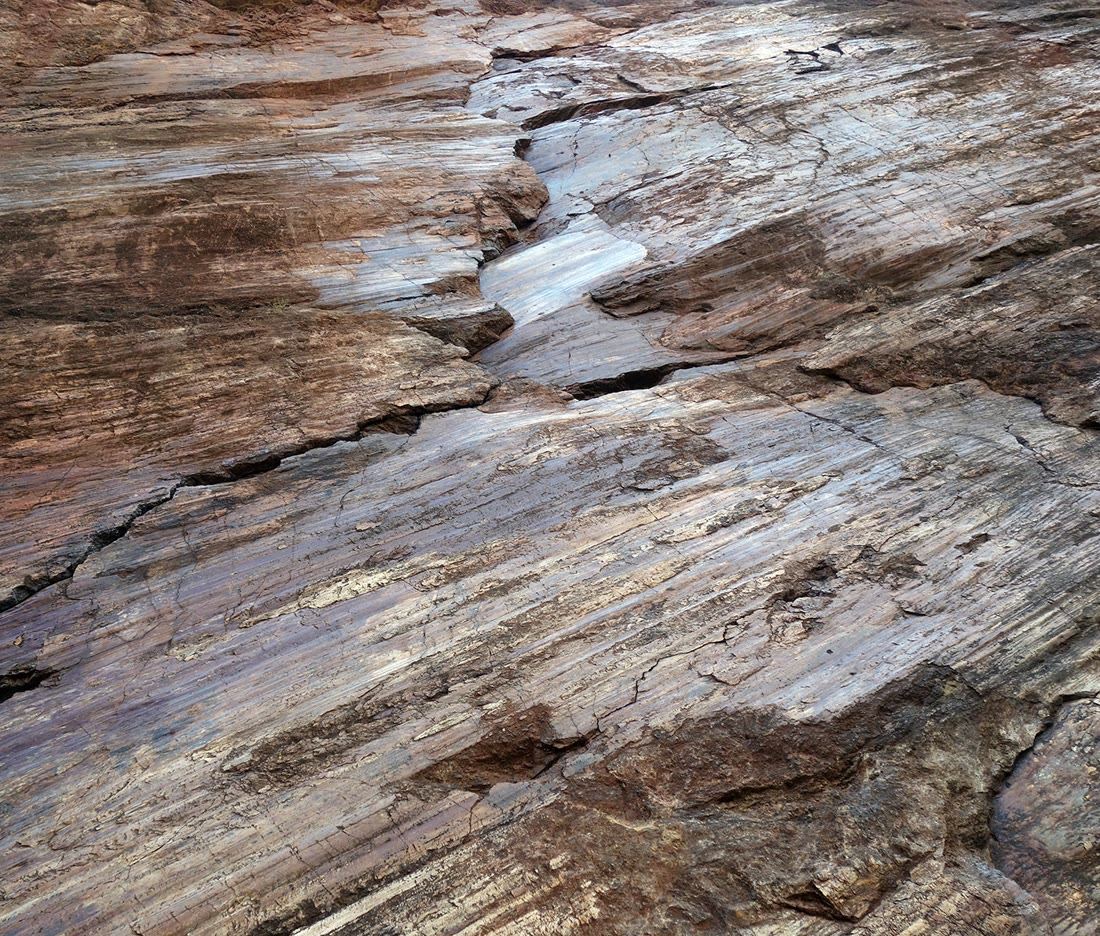
\includegraphics[height=5.2cm]{images/book3/b1-slickenside.jpg}\hfill
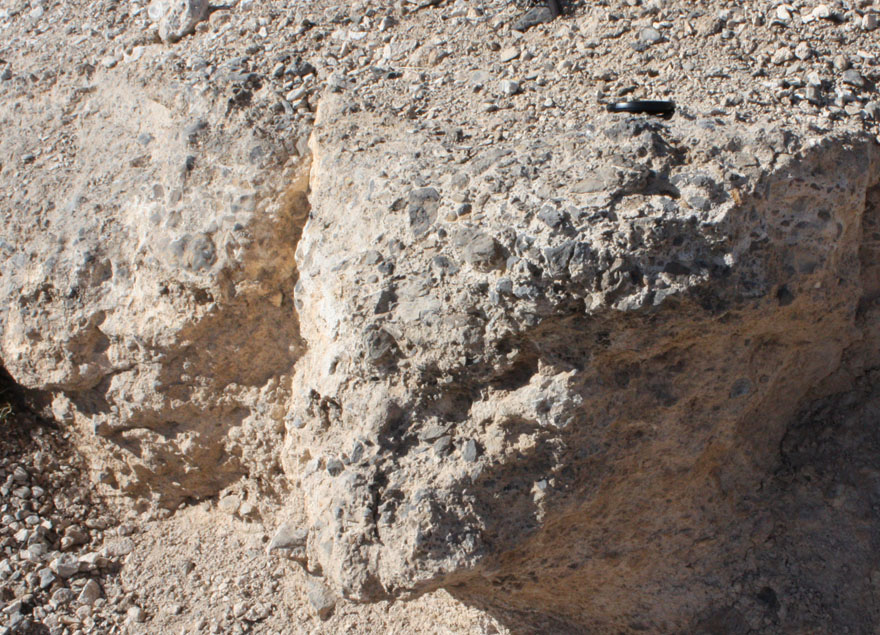
\includegraphics[height=5.2cm]{images/book3/b1-fault-breccia.jpg}
\par\smallskip{\small Links: een \omterm{def:b1:faults-folds-fabrics:fault-rocks}{slickenside} op een breukvlak in chert, van ongeveer \qtyproduct{3 x 3}{m} van een vlak van \qty{10}{m} hoog, Corona Heights, San Francisco; het gepolijste vlak is langs de verschuiving gestrieerd. Foto: Dextersinister, CC~BY-SA~4.0. Rechts: \omterm{def:b1:faults-folds-fabrics:fault-rocks}{breukbreccie} van de \omterm{def:b1:faults-folds-fabrics:fault-types}{Keystone-overschuiving}, Red Rock Canyon, Nevada: hoekige fragmenten van grijs carbonaatgesteente in een lichtere matrix; de lensdop rechtsboven is \qty{5.8}{cm} breed. Foto: Jstuby, publiek domein. Beide van Wikimedia Commons.}
\label{fig:b1:faults-folds-fabrics:fault-surfaces}
\end{omfigure}
% ledger: commons:slickenside, commons:breccia

\begin{method}[Het meten van de verschuiving op een breuk]\label{met:b1:faults-folds-fabrics:slip}
\begin{enumerate}
  \item Meet de ligging $\alpha/\delta$ van het breukvlak en schrijf zijn \omterm{def:b1:geological-maps:attitude}{strijk}, $\alpha - \ang{90}$, op.
  \item Meet de \omterm{def:b1:faults-folds-fabrics:fault-rocks}{slickenlines}: hun \omterm{def:b1:faults-folds-fabrics:fault-elements}{rake} op de breuk, of hun richting en \omterm{def:b1:field-lab-methods-1:trend-plunge}{duik}; voor een \omterm{def:b1:faults-folds-fabrics:fault-elements}{rake} $r$ geldt $\sin p = |\sin r|\sin\delta$.
  \item Bepaal in welke richting de \omterm{def:b1:faults-folds-fabrics:fault-elements}{hangende wand} is bewogen, uit merkers die over de breuk zijn verspringen, en geef de \omterm{def:b1:faults-folds-fabrics:fault-elements}{rake} haar teken: negatief als de \omterm{def:b1:faults-folds-fabrics:fault-elements}{hangende wand} omlaag is gegaan.
  \item Bepaal de \omterm{def:b1:faults-folds-fabrics:fault-elements}{netto verschuiving} $L$ uit twee punten die ooit één waren; als alleen de \omterm{def:b1:cross-sections:throw}{worp} $h$ van een horizontale merker bekend is, geldt $L = h/(|\sin r|\sin\delta)$.
  \item Bereken de componenten met \cref{prop:b1:faults-folds-fabrics:slip-components} en noem de breuk met \cref{def:b1:faults-folds-fabrics:fault-types}.
\end{enumerate}
\end{method}

\begin{inthefield}[Een breukvlak meten]
Een geoloog die in een \omterm{def:b1:geological-maps:geological-map}{ontsluiting} een breukvlak vindt, meet het zoals elk ander vlak, met een kompas-kliseometer op het vlak gelegd, en meet daarna de \omterm{def:b1:faults-folds-fabrics:fault-rocks}{slickenlines} erop, hetzij als \omterm{def:b1:faults-folds-fabrics:fault-elements}{rake}, met een geodriehoek op het vlak gelegd, hetzij als richting en \omterm{def:b1:field-lab-methods-1:trend-plunge}{duik}. De twee worden met elkaar gecontroleerd met de formule van stap~2 van de methode. De zin van de beweging is het moeilijke deel. Kleine treden op een \omterm{def:b1:faults-folds-fabrics:fault-rocks}{slickenside}, en vezels van kwarts of calciet die groeiden terwijl de blokken uiteengingen, kunnen aantonen welke kant het ontbrekende blok op ging, maar sommige treden wijzen de verkeerde kant op, dus wordt de zin alleen vertrouwd wanneer hij overeenkomt met de verspringing van een merkerlaag of een ader. \omterm{def:b1:faults-folds-fabrics:fault-rocks}{Breukgesteenten} worden beschreven en bemonsterd, en een \omterm{def:b1:rifts-ridges-margins:transform}{breukzone} die te breed is om op één plaats te meten, wordt als band in kaart gebracht. Elke breuk wordt genoteerd op een genummerd station van het notitieboek, met haar ligging, haar \omterm{def:b1:faults-folds-fabrics:fault-rocks}{slickenlines}, de zin van de beweging en hoe zeker de geoloog daarvan is.
\end{inthefield}

\section{Andersons theorie van de breuken}\label{sec:b1:faults-folds-fabrics:anderson}

Waarom zijn de meeste \omterm{def:b1:faults-folds-fabrics:fault-types}{normaalbreuken} steil en de meeste \omterm{def:b1:faults-folds-fabrics:fault-types}{overschuivingen} flauw? In 1905 antwoordde de Schotse geoloog Ernest Masson Anderson met twee opmerkingen: het oppervlak van de Aarde bepaalt de richtingen van de \omterm{def:b1:stress-strain-rheology:principal}{hoofdspanningen}, en het Coulomb-criterium bepaalt dan de hoek van de breuken.
% ledger: ws:anderson, anderson:1905

\begin{proposition}[Een vrij oppervlak maakt een hoofdvlak]\label{prop:b1:faults-folds-fabrics:free-surface}
Aan het oppervlak van de Aarde, waar het horizontaal is, is één hoofdspanning verticaal en zijn de twee andere horizontaal.
\end{proposition}

\begin{proof}
De lucht drukt op de grond alleen met haar druk, loodrecht op het oppervlak: zij oefent geen schuifspanning uit. De spanning op het horizontale vlak aan het oppervlak staat daarom loodrecht erop. In drie dimensies is de spanning op een vlak met eenheidsnormaal $\mathbf n$ de vector $\boldsymbol\sigma\mathbf n$ (natuurkundeboeken, derde jaar); heeft zij geen schuifdeel, dan is zij evenwijdig aan $\mathbf n$, zodat $\boldsymbol\sigma\mathbf n = \lambda\mathbf n$ en $\mathbf n$ een eigenvector is van de symmetrische matrix $\boldsymbol\sigma$: een hoofdrichting (\cref{def:b1:stress-strain-rheology:principal}). De verticale is dus een hoofdrichting, en de twee andere, loodrecht erop, zijn horizontaal.
\end{proof}

Anderson nam aan dat de \omterm{def:b1:stress-strain-rheology:principal}{hoofdspanningen} deze richtingen behouden tot op de diepten waarop breuken ontstaan. De aanname geldt goed onder een flauw hellend oppervlak en in gesteenten zonder sterke oude zwakke zones; zij faalt bij steil reliëf en waar oude breuken of lagen de nieuwe sturen. Met haar zijn slechts drie gevallen mogelijk, naargelang welke van $\sigma_1$, $\sigma_2$ en $\sigma_3$ verticaal is.

\begin{theorem}[Andersons theorie van de breuken]\label{thm:b1:faults-folds-fabrics:anderson}
Laat één hoofdspanning verticaal zijn en laat het gesteente breken volgens het Coulomb-criterium, met \omterm{def:b1:stress-strain-rheology:coulomb}{inwendige wrijvingshoek} $\phi$. Nieuwe breuken vormen zich op vlakken die de richting van $\sigma_2$ bevatten en de hoek $\ang{45} - \phi/2$ maken met $\sigma_1$, en zij schuiven loodrecht op $\sigma_2$, waarbij het gesteente langs $\sigma_1$ wordt verkort. Dus
\begin{enumerate}[label=(\alph*)]
  \item als $\sigma_1$ verticaal is, ontstaan \omterm{def:b1:faults-folds-fabrics:fault-types}{normaalbreuken}, lopend langs $\sigma_2$ en met een helling van $\ang{45} + \phi/2$;
  \item als $\sigma_3$ verticaal is, ontstaan \omterm{def:b1:faults-folds-fabrics:fault-types}{overschuivingen}, lopend langs $\sigma_2$ en met een helling van $\ang{45} - \phi/2$;
  \item als $\sigma_2$ verticaal is, ontstaan verticale \omterm{def:b1:faults-folds-fabrics:fault-types}{strike-slip-breuken}, die lopen onder $\ang{45} - \phi/2$ aan weerszijden van $\sigma_1$.
\end{enumerate}
Met $\phi = \ang{30}$ zijn de hellingen \ang{60}, \ang{30} en \ang{90}.
\end{theorem}
\index{Andersons theorie van de breuken}

\begin{proof}
Op een vlak dat de richting van $\sigma_2$ bevat, ligt de normaal in het vlak van $\sigma_1$ en $\sigma_3$, en is de spanning op het vlak die van het tweedimensionale probleem van \cref{ch:b1:stress-strain-rheology}: haar punt ligt op de cirkel van Mohr van $\sigma_1$ en $\sigma_3$, en haar schuifdeel ligt in het vlak van $\sigma_1$ en $\sigma_3$, loodrecht op $\sigma_2$. Op elk
ander vlak ligt het punt $(\sigma_n, \tau)$ binnen die cirkel, die de grootste is van de drie cirkels van Mohr van een driedimensionale spanningstoestand (aangenomen uit de driedimensionale theorie). Naarmate de spanningen groeien, raakt de Coulomb-lijn dus eerst aan vlakken die $\sigma_2$ bevatten, en onder hen, volgens \cref{thm:b1:stress-strain-rheology:failure-angle}, aan die onder $\ang{45} - \phi/2$ met $\sigma_1$. Schuiven op zo'n vlak, loodrecht op $\sigma_2$, brengt de twee blokken langs de richting van de grootste compressie dichter bij elkaar en verwijdert ze langs de kleinste, zoals het moet om de spanning te ontlasten. In geval (a) maakt het vlak de hoek $\ang{45} - \phi/2$ met de verticale, dus het helt onder $\ang{45} + \phi/2$; het loopt langs de horizontale $\sigma_2$; de verschuiving ligt in het verticale vlak van de helling, en het blok erboven gaat omlaag, waardoor het gesteente horizontaal wordt verlengd: een \omterm{def:b1:faults-folds-fabrics:fault-types}{normaalbreuk}. In geval (b) maakt het vlak $\ang{45} - \phi/2 < \ang{45}$ met de horizontale $\sigma_1$, en verkort de verschuiving het gesteente horizontaal, en duwt zij de \omterm{def:b1:faults-folds-fabrics:fault-elements}{hangende wand} omhoog: een \omterm{def:b1:faults-folds-fabrics:fault-types}{overschuiving}. In geval (c) bevatten de vlakken de verticale, dus zijn zij verticaal; de verschuiving is horizontaal, loodrecht op $\sigma_2$: \omterm{def:b1:faults-folds-fabrics:fault-types}{strike-slip-breuken}, onder $\ang{45} - \phi/2$ aan weerszijden van de horizontale $\sigma_1$.
\end{proof}

In elk regime zijn twee stelsels breuken mogelijk, symmetrisch rond $\sigma_1$: geconjugeerde breuken, die samenkomen onder $\ang{90} - \phi$, ongeveer \ang{60}, met $\sigma_1$ in de scherpe hoek tussen hen. Omgekeerd geeft een paar geconjugeerde breuken dat in het veld wordt gemeten de richtingen van de spanningen die ze maakten: $\sigma_1$ halveert hun scherpe hoek, $\sigma_2$ is hun snijlijn.

\begin{omfigure}
\begin{tikzpicture}[x={(1cm,0cm)}, y={(0.42cm,0.30cm)}, z={(0cm,1cm)},
  >={Stealth[length=5pt]}, font=\small, scale=0.86,
  face/.style={draw=black, line width=0.5pt, line join=round},
  sone/.style={->, line width=1.6pt, omThm},
  sthree/.style={->, line width=0.8pt, omDef}]
% exact geometry: the fault plane is X = xf(Z); slip is along the dip; throw t
% (a) normal fault: dip 60, xf(Z) = 1.3 + (1.6 - Z)/tan 60, throw 0.45
\begin{scope}
  \def\W{3.2}\def\D{1.6}\def\H{1.6}
  \pgfmathsetmacro{\c}{1/tan(60)}
  \pgfmathsetmacro{\xa}{1.3+1.6*\c}       % xf(0)
  \pgfmathsetmacro{\xb}{1.3+0.45*\c}      % xf(H - t)
  \pgfmathsetmacro{\mfa}{1.3+(1.6-0.55)*\c}\pgfmathsetmacro{\mfb}{1.3+(1.6-0.85)*\c}
  \pgfmathsetmacro{\mha}{1.3+(1.6-0.10)*\c}\pgfmathsetmacro{\mhb}{1.3+(1.6-0.40)*\c}
  % footwall
  \fill[omLithSand!55] (0,0,0) -- (\xa,0,0) -- (1.3,0,\H) -- (0,0,\H) -- cycle;
  \fill[omProp!40] (0,0,0.55) -- (\mfa,0,0.55) -- (\mfb,0,0.85) -- (0,0,0.85) -- cycle;
  \draw[face] (0,0,0) -- (\xa,0,0) -- (1.3,0,\H) -- (0,0,\H) -- cycle;
  \draw[face, fill=omLithSand!35] (0,0,\H) -- (1.3,0,\H) -- (1.3,\D,\H) -- (0,\D,\H) -- cycle;
  \draw[face, fill=black!12] (1.3,0,\H) -- (\xb,0,1.15) -- (\xb,\D,1.15) -- (1.3,\D,\H) -- cycle;
  % hanging wall
  \fill[omLithSand!55] (\xa,0,0) -- (\W,0,0) -- (\W,0,1.15) -- (\xb,0,1.15) -- cycle;
  \fill[omProp!40] (\mha,0,0.10) -- (\W,0,0.10) -- (\W,0,0.40) -- (\mhb,0,0.40) -- cycle;
  \draw[face] (\xa,0,0) -- (\W,0,0) -- (\W,0,1.15) -- (\xb,0,1.15) -- cycle;
  \draw[face, fill=omLithSand!35] (\xb,0,1.15) -- (\W,0,1.15) -- (\W,\D,1.15) -- (\xb,\D,1.15) -- cycle;
  \fill[omLithSand!45] (\W,0,0) -- (\W,\D,0) -- (\W,\D,1.15) -- (\W,0,1.15) -- cycle;
  \fill[omProp!30] (\W,0,0.10) -- (\W,\D,0.10) -- (\W,\D,0.40) -- (\W,0,0.40) -- cycle;
  \draw[face] (\W,0,0) -- (\W,\D,0) -- (\W,\D,1.15) -- (\W,0,1.15) -- cycle;
  % slip arrow on the front face
  \draw[->, line width=0.9pt] (1.45,0,1.05) -- ++({0.35*cos(60)},0,{-0.35*sin(60)});
  % stresses: sigma1 vertical, sigma3 horizontal across the strike
  \draw[sone] (1.6,0.8,3.05) -- (1.6,0.8,2.1) node[pos=0, left] {$\sigma_1$};
  \draw[sone] (1.6,0.8,-1.1) -- (1.6,0.8,-0.15);
  \draw[sthree] (-0.85,0.8,0.8) -- (-0.15,0.8,0.8) node[pos=0, above] {$\sigma_3$};
  \draw[sthree] (4.05,0.8,0.6) -- (3.35,0.8,0.6);
  \node[font=\small\bfseries] at (1.9,0,-1.55) {(a) normaalbreuk};
\end{scope}
% (b) thrust fault: dip 30, xf(Z) = 3.0 - Z/tan 30, throw 0.35, heave 0.606
\begin{scope}[xshift=6.0cm]
  \def\D{1.6}\def\H{1.3}
  \pgfmathsetmacro{\c}{1/tan(30)}
  \pgfmathsetmacro{\Wp}{4.0-0.35*\c}       % right face of the hanging wall
  \pgfmathsetmacro{\xt}{3.0-1.3*\c}        % footwall top edge
  \pgfmathsetmacro{\xh}{3.0-1.65*\c}       % hanging-wall top edge
  \pgfmathsetmacro{\mfa}{3.0-0.50*\c}\pgfmathsetmacro{\mfb}{3.0-0.75*\c}
  \pgfmathsetmacro{\mha}{3.0-0.85*\c}\pgfmathsetmacro{\mhb}{3.0-1.10*\c}
  % footwall
  \fill[omLithSand!55] (0,0,0) -- (3.0,0,0) -- (\xt,0,\H) -- (0,0,\H) -- cycle;
  \fill[omProp!40] (0,0,0.50) -- (\mfa,0,0.50) -- (\mfb,0,0.75) -- (0,0,0.75) -- cycle;
  \draw[face] (0,0,0) -- (3.0,0,0) -- (\xt,0,\H) -- (0,0,\H) -- cycle;
  \draw[face, fill=omLithSand!35] (0,0,\H) -- (\xt,0,\H) -- (\xt,\D,\H) -- (0,\D,\H) -- cycle;
  % hanging wall
  \fill[omLithSand!55] (3.0,0,0) -- (\Wp,0,0) -- (\Wp,0,1.65) -- (\xh,0,1.65) -- cycle;
  \fill[omProp!40] (\mha,0,0.85) -- (\Wp,0,0.85) -- (\Wp,0,1.10) -- (\mhb,0,1.10) -- cycle;
  \draw[face] (3.0,0,0) -- (\Wp,0,0) -- (\Wp,0,1.65) -- (\xh,0,1.65) -- cycle;
  \draw[face, fill=omLithSand!35] (\xh,0,1.65) -- (\Wp,0,1.65) -- (\Wp,\D,1.65) -- (\xh,\D,1.65) -- cycle;
  \fill[omLithSand!45] (\Wp,0,0) -- (\Wp,\D,0) -- (\Wp,\D,1.65) -- (\Wp,0,1.65) -- cycle;
  \fill[omProp!30] (\Wp,0,0.85) -- (\Wp,\D,0.85) -- (\Wp,\D,1.10) -- (\Wp,0,1.10) -- cycle;
  \draw[face] (\Wp,0,0) -- (\Wp,\D,0) -- (\Wp,\D,1.65) -- (\Wp,0,1.65) -- cycle;
  \draw[->, line width=0.9pt] (2.25,0,0.62) -- ++({-0.42*cos(30)},0,{0.42*sin(30)});
  % stresses: sigma1 horizontal across the strike, sigma3 vertical
  \draw[sone] (-1.2,0.8,0.65) -- (-0.15,0.8,0.65) node[pos=0, above] {$\sigma_1$};
  \draw[sone] (\Wp+1.15,0.8,0.45) -- (\Wp+0.1,0.8,0.45);
  \draw[sthree] (2.0,0.8,2.7) -- (2.0,0.8,2.0) node[pos=0, left] {$\sigma_3$};
  \draw[sthree] (2.0,0.8,-0.9) -- (2.0,0.8,-0.2);
  \node[font=\small\bfseries] at (2.0,0,-1.55) {(b) overschuiving};
\end{scope}
% (c) strike-slip fault: vertical, along the y axis at X = 1.6; dextral: the far
% (east) block has moved toward the reader by 0.5; sigma1 at 30 deg clockwise of the strike
\begin{scope}[xshift=12.0cm]
  \def\D{2.2}\def\H{1.1}\def\s{0.5}
  % west block
  \draw[face, fill=omLithSand!55] (0,0,0) -- (1.6,0,0) -- (1.6,0,\H) -- (0,0,\H) -- cycle;
  \draw[face, fill=omLithSand!35] (0,0,\H) -- (1.6,0,\H) -- (1.6,\D,\H) -- (0,\D,\H) -- cycle;
  \draw[face, fill=black!12] (1.6,\D-\s,0) -- (1.6,\D,0) -- (1.6,\D,\H) -- (1.6,\D-\s,\H) -- cycle;
  \draw[line width=1.4pt, omProp] (0,1.25,\H) -- (1.6,1.25,\H);
  % east block
  \draw[face, fill=omLithSand!55] (1.6,-\s,0) -- (3.2,-\s,0) -- (3.2,-\s,\H) -- (1.6,-\s,\H) -- cycle;
  \draw[face, fill=omLithSand!35] (1.6,-\s,\H) -- (3.2,-\s,\H) -- (3.2,\D-\s,\H) -- (1.6,\D-\s,\H) -- cycle;
  \draw[face, fill=omLithSand!45] (3.2,-\s,0) -- (3.2,\D-\s,0) -- (3.2,\D-\s,\H) -- (3.2,-\s,\H) -- cycle;
  \draw[line width=1.4pt, omProp] (1.6,1.25-\s,\H) -- (3.2,1.25-\s,\H);
  % slip arrows on the top
  \draw[->, line width=0.9pt] (2.05,1.35,\H) -- (2.05,0.35,\H);
  \draw[->, line width=0.9pt] (1.15,0.55,\H) -- (1.15,1.55,\H);
  % stresses in the horizontal plane, drawn at the height of the top surface
  \draw[sone] ({1.6+1.9*sin(30)},{0.8+1.9*cos(30)},\H) -- ({1.6+1.0*sin(30)},{0.8+1.0*cos(30)},\H) node[pos=0, right] {$\sigma_1$};
  \draw[sone] ({1.6-1.9*sin(30)},{0.8-1.9*cos(30)},\H) -- ({1.6-1.0*sin(30)},{0.8-1.0*cos(30)},\H);
  \draw[sthree] ({1.6+2.0*sin(120)},{0.8+2.0*cos(120)},\H) -- ({1.6+1.45*sin(120)},{0.8+1.45*cos(120)},\H) node[pos=0, right] {$\sigma_3$};
  \draw[sthree] ({1.6-2.0*sin(120)},{0.8-2.0*cos(120)},\H) -- ({1.6-1.45*sin(120)},{0.8-1.45*cos(120)},\H);
  \node[font=\small\bfseries] at (1.7,0,-1.55) {(c) strike-slip-breuk};
\end{scope}
\end{tikzpicture}
\par\smallskip{\small De drie regimes van Anderson, met de breuken onder de hellingen van de stelling voor $\phi = \ang{30}$: \ang{60}, \ang{30} en verticaal. Dikke rode pijlen: $\sigma_1$; dunne blauwe pijlen: $\sigma_3$; $\sigma_2$ loopt langs de \omterm{def:b1:geological-maps:attitude}{strijk} van de breuken in (a) en (b) en is verticaal in (c). Een merkerlaag (oranje) is in (a) en (b) over de \omterm{def:b1:cross-sections:throw}{worp} verschoven; in (c) is een lijn op de grond horizontaal verschoven, en de breuk is \omterm{def:b1:faults-folds-fabrics:fault-types}{dextraal}: vanuit elk blok gezien is het andere naar rechts bewogen. De zwarte pijlen geven de verschuiving aan.}
\label{fig:b1:faults-folds-fabrics:anderson}
\end{omfigure}

De drie regimes komen overeen met de drie soorten plaatgrens van \cref{ch:b1:rifts-ridges-margins,ch:b1:active-margins}. Waar de \omterm{def:b1:layered-earth:lithosphere}{lithosfeer} wordt uitgerekt, bij riften en ruggen, daalt de horizontale spanning onder de verticale en ontstaan \omterm{def:b1:faults-folds-fabrics:fault-types}{normaalbreuken}; waar zij wordt samengedrukt, bij convergente randen en in bergketens, overschrijdt de horizontale spanning het gewicht van de rots en ontstaan \omterm{def:b1:faults-folds-fabrics:fault-types}{overschuivingen}; langs \omterm{def:b1:rifts-ridges-margins:transform}{transformbreuken} omsluiten de twee horizontale spanningen de verticale. De hellingen passen op een ruwe manier bij de waarnemingen: de \omterm{def:b1:faults-folds-fabrics:fault-types}{normaalbreuken} van riften helen dicht bij het oppervlak rond \ang{60}, en \omterm{def:b1:faults-folds-fabrics:fault-types}{overschuivingen} zijn \omterm{def:b1:faults-folds-fabrics:fault-types}{omgekeerde breuken} met een kleine hoek. De uitzonderingen zijn leerzaam. Veel \omterm{def:b1:faults-folds-fabrics:fault-types}{normaalbreuken} worden met de diepte vlakker, en sommige doorsneden van riften tonen ze tot in een bijna vlakke zone van schuiving: deze \omterm{def:b1:faults-folds-fabrics:fault-types}{normaalbreuken} met kleine hoek, of detachments, snijden de \omterm{def:b1:layered-earth:layers}{korst} onder ruim \ang{45}. De theorie van Anderson kan ze niet als nieuwe breuken verklaren, en \cref{exo:b1:faults-folds-fabrics:10} laat zien dat de wrijving van Byerlee ze onder Andersoniaanse spanningen evenmin kan laten glijden: zij hebben zwakke \omterm{def:b1:faults-folds-fabrics:fault-rocks}{breukgesteenten}, een hoge poriëndruk of gedraaide spanningen nodig. Een breuk die al bestaat, glijdt bij de wrijving van de \omterm{prop:b1:stress-strain-rheology:byerlee}{wet van Byerlee}, $\mu = 0.85$, $\phi = \ang{40.4}$; de best georiënteerde \omterm{def:b1:faults-folds-fabrics:fault-types}{normaalbreuken} helen dan onder \ang{65.2}, zoals het probleem van \cref{ch:b1:stress-strain-rheology} vond.
% ledger: ws:anderson, usgs:fault-types, byerlee:1975

\begin{history}[De breuken van Anderson]
Ernest Masson Anderson, een Schotse geoloog, publiceerde zijn theorie van de drie soorten breuken in 1905, in een korte verhandeling over de dynamiek van breukvorming, en gaf haar volledige vorm, met de toepassing op de gangen en breuken van Groot-Brittannië, in zijn boek \emph{The Dynamics of Faulting and Dyke Formation}. Een klein aantal artikelen en dat boek bepalen nog steeds de structurele geologie, de seismologie en de rotsmechanica: zijn drie regimes, normaal, \omterm{def:b1:faults-folds-fabrics:fault-types}{overschuiving} en strike-slip, zijn de gebruikelijke manier om spanningstoestanden in de \omterm{def:b1:layered-earth:layers}{korst} en de breuken die zij maken te sorteren, en om de spanning uit de breuken af te lezen.
\end{history}
% ledger: anderson:1905, healy:anderson, ws:anderson

\section{Plooigeometrie}\label{sec:b1:faults-folds-fabrics:folds}

\Cref{ch:b1:geological-maps} noemde \omterm{def:b1:geological-maps:fold}{plooien} en las hun patronen op kaarten. In drie dimensies heeft een \omterm{def:b1:geological-maps:fold}{plooi} meer namen nodig: waar zij buigt, hoe scherp, en hoe zij in de ruimte is gelegen.

\begin{definition}[Scharnier, scharnierlijn, flank, axiaal vlak, interflankhoek, cilindrische plooi]\label{def:b1:faults-folds-fabrics:fold-elements}
Op een geplooid oppervlak is het \emph{scharnier}\index{scharnier (van een plooi)} de zone van grootste kromming en de \emph{scharnierlijn}\index{scharnierlijn} de lijn die haar punten van grootste kromming verbindt; de \emph{flanken}\index{flank (van een plooi)} zijn de minder gekromde delen aan weerszijden. Het axiale oppervlak van een \omterm{def:b1:geological-maps:fold}{plooi} is het oppervlak dat de scharnierlijnen van haar opeenvolgende geplooide oppervlakken verbindt;
wanneer het een vlak is, is het het \emph{axiaal vlak}\index{axiaal vlak}. De \emph{interflankhoek}\index{interflankhoek} $\iota$ is de hoek tussen de twee flanken, gemeten in het profiel, het vlak loodrecht op de scharnierlijn, tussen de raaklijnen aan de flanken in hun buigpunten;
$0 \le \iota \le \ang{180}$. Een \omterm{def:b1:geological-maps:fold}{plooi} is een \emph{cilindrische plooi}\index{cilindrische plooi} wanneer haar oppervlakken worden voortgebracht door een rechte lijn die evenwijdig aan zichzelf wordt verplaatst; de richting van die lijn is de \omterm{def:b1:geological-maps:fold}{plooias} van \cref{def:b1:geological-maps:fold}, en elke scharnierlijn van een cilindrische \omterm{def:b1:geological-maps:fold}{plooi} is een rechte lijn evenwijdig eraan.
\end{definition}
% ledger: ws:fold-elements

\begin{omfigure}
\begin{tikzpicture}[x={(1cm,0cm)}, y={(0.42cm,0.30cm)}, z={(0cm,1cm)},
  >={Stealth[length=5pt]}, font=\small, scale=1.15]
% a cylindrical anticline: the top of a bed is z = f(x) = 0.35 a - a sqrt(x^2 + 0.35^2), a = tan 50
% (limbs dip toward 50 deg, interlimb angle 80 deg); the bed is 0.7 thick, measured vertically
% (a similar fold); the fold axis is the y direction, horizontal.
\def\D{2.8}
\pgfmathsetmacro{\a}{tan(50)}
\def\f(#1){0.35*\a - \a*sqrt((#1)*(#1) + 0.1225)}
\pgfmathsetmacro{\zt}{0.35*\a}
% top surface of the bed
\fill[omLithSand!35] plot[domain=-1.7:1.7, samples=61, variable=\x] (\x, 0, {\f(\x)})
  -- plot[domain=1.7:-1.7, samples=61, variable=\x] (\x, \D, {\f(\x)}) -- cycle;
\foreach \u in {-1.4,-1.0,-0.6,-0.3,0.3,0.6,1.0,1.4} {
  \draw[black!35, line width=0.3pt] (\u, 0, {\f(\u)}) -- (\u, \D, {\f(\u)});
}
\draw[line width=0.5pt] plot[domain=-1.7:1.7, samples=61, variable=\x] (\x, \D, {\f(\x)});
\draw[line width=0.5pt] (-1.7, 0, {\f(-1.7)}) -- (-1.7, \D, {\f(-1.7)});
% right end face
\fill[omLithSand!55] (1.7, 0, {\f(1.7)}) -- (1.7, \D, {\f(1.7)}) -- (1.7, \D, {\f(1.7)-0.7}) -- (1.7, 0, {\f(1.7)-0.7}) -- cycle;
\draw[line width=0.5pt] (1.7, 0, {\f(1.7)}) -- (1.7, \D, {\f(1.7)}) -- (1.7, \D, {\f(1.7)-0.7}) -- (1.7, 0, {\f(1.7)-0.7});
% axial plane, behind the front face
\fill[omDef!30, opacity=0.5] (0, 0, 0.85) -- (0, \D, 0.85) -- (0, \D, -2.0) -- (0, 0, -2.0) -- cycle;
\draw[omDef, line width=0.6pt] (0, 0, -2.0) -- (0, 0, 0.85) -- (0, \D, 0.85) -- (0, \D, -2.0);
% hinge line
\draw[omThm, line width=1.5pt] (0, 0, 0) -- (0, \D, 0);
% front face of the bed (the profile)
\fill[omLithSand!80] plot[domain=-1.7:1.7, samples=61, variable=\x] (\x, 0, {\f(\x)})
  -- plot[domain=1.7:-1.7, samples=61, variable=\x] (\x, 0, {\f(\x)-0.7}) -- cycle;
\draw[line width=0.7pt] plot[domain=-1.7:1.7, samples=61, variable=\x] (\x, 0, {\f(\x)});
\draw[line width=0.7pt] plot[domain=-1.7:1.7, samples=61, variable=\x] (\x, 0, {\f(\x)-0.7});
\draw[line width=0.5pt] (-1.7, 0, {\f(-1.7)}) -- (-1.7, 0, {\f(-1.7)-0.7});
\draw[omDef, line width=0.6pt, dashed] (0, 0, 0) -- (0, 0, -0.7);
\draw[omDef, line width=0.6pt] (0, 0, -0.7) -- (0, 0, -2.0);
% interlimb angle on the profile, in the core: tangents to the limbs of the base of the bed
% meet at (0, 0, zt - 0.7)
\pgfmathsetmacro{\zb}{\zt-0.7}
\draw[black!70, dashed] (-1.3, 0, {\zb-1.3*\a}) -- (0, 0, \zb) -- (1.3, 0, {\zb-1.3*\a});
\draw[black, line width=0.5pt] plot[domain=-140:-40, samples=21, variable=\t] ({0.75*cos(\t)}, 0, {\zb+0.75*sin(\t)});
\node[font=\scriptsize] at (0.22, 0, {\zb-1.0}) {$\iota$};
% labels
\node[omThm, anchor=west, font=\scriptsize] at (0.08, \D, 0.1) {scharnierlijn};
\node[omDef, anchor=south, font=\scriptsize] at (0, \D, 0.85) {axiaal vlak};
\node[font=\scriptsize, rotate=50] at (-1.15, 0, {\f(-1.15)-0.35}) {flank};
\node[font=\scriptsize, rotate=-50] at (1.15, 0, {\f(1.15)-0.35}) {flank};
\end{tikzpicture}
\par\smallskip{\small De elementen van een cilindrische \omterm{def:b1:geological-maps:fold}{antiklinaal}, hier met een horizontale \omterm{def:b1:faults-folds-fabrics:fold-elements}{scharnierlijn}: het \omterm{def:b1:faults-folds-fabrics:fold-elements}{scharnier}, waar de laag het sterkst buigt; de twee \omterm{def:b1:faults-folds-fabrics:fold-elements}{flanken}; het axiale vlak door de \omterm{def:b1:faults-folds-fabrics:fold-elements}{scharnierlijnen} van de bovenkant en de onderkant van de laag; en de \omterm{def:b1:faults-folds-fabrics:fold-elements}{interflankhoek} $\iota$ tussen de raaklijnen aan de \omterm{def:b1:faults-folds-fabrics:fold-elements}{flanken}, gemeten in het profiel vooraan, hier \ang{80}, op de onderkant van de laag getekend. De grijze lijnen op de bovenkant van de laag zijn evenwijdig aan de \omterm{def:b1:geological-maps:fold}{plooias}.}
\label{fig:b1:faults-folds-fabrics:fold-elements}
\end{omfigure}

Wanneer de \omterm{def:b1:faults-folds-fabrics:fold-elements}{flanken} vlakken zijn, zoals in de chevronplooien hieronder en in de Varden Hills, volgt de meetkunde van een \omterm{def:b1:geological-maps:fold}{plooi} uit de ligging van haar \omterm{def:b1:faults-folds-fabrics:fold-elements}{flanken}. De opwaartse eenheidsnormaal van een vlak met \omterm{def:b1:geological-maps:attitude}{helling-richting} $\alpha$ en helling $\delta$ is $\mathbf n = (\sin\delta\sin\alpha, \sin\delta\cos\alpha, \cos\delta)$, in oost-, noord- en opwaartse componenten.

\begin{proposition}[Een plooi uit haar flanken]\label{prop:b1:faults-folds-fabrics:hinge}
Laat een \omterm{def:b1:faults-folds-fabrics:fold-elements}{cilindrische plooi} vlakke \omterm{def:b1:faults-folds-fabrics:fold-elements}{flanken} hebben, geen van beide overgekanteld, met opwaartse eenheidsnormalen $\mathbf n_1$ en $\mathbf n_2$. Haar \omterm{def:b1:faults-folds-fabrics:fold-elements}{scharnierlijn} is evenwijdig aan $\mathbf n_1 \times \mathbf n_2$, en haar \omterm{def:b1:faults-folds-fabrics:fold-elements}{interflankhoek} is
\[
  \iota = \ang{180} - \arccos(\mathbf n_1\cdot\mathbf n_2) .
\]
\end{proposition}

\begin{proof}
Elke flank wordt voortgebracht door lijnen evenwijdig aan de \omterm{def:b1:geological-maps:fold}{plooias}, dus bevat zij de richting van de as, die daarom loodrecht staat op beide normalen en evenwijdig is aan hun uitwendig product; de \omterm{def:b1:faults-folds-fabrics:fold-elements}{scharnierlijn} is evenwijdig aan de as. Het profiel staat loodrecht op de as, dus het bevat beide normalen; daarin verschijnen de twee \omterm{def:b1:faults-folds-fabrics:fold-elements}{flanken} als twee lijnen loodrecht op $\mathbf n_1$ en $\mathbf n_2$, en de hoek tussen de lijnen is gelijk aan de hoek $\arccos(\mathbf n_1\cdot\mathbf n_2)$ tussen de normalen of aan haar supplement. Wanneer de lagen niet geplooid zijn, vallen de twee normalen samen en is de \omterm{def:b1:faults-folds-fabrics:fold-elements}{interflankhoek} \ang{180}; wanneer de \omterm{def:b1:faults-folds-fabrics:fold-elements}{flanken} draaien, groeit de hoek tussen de normalen vanaf $0$ terwijl de \omterm{def:b1:faults-folds-fabrics:fold-elements}{interflankhoek} afneemt vanaf \ang{180}, zodat de twee samen \ang{180} blijven geven zolang beide normalen omhoog wijzen.
\end{proof}

Voor een \omterm{def:b1:faults-folds-fabrics:fold-classes}{rechtopstaande plooi} waarvan de twee \omterm{def:b1:faults-folds-fabrics:fold-elements}{flanken} aan weerszijden $\delta$ helen, maken de normalen de hoek $2\delta$ en $\iota = \ang{180} - 2\delta$.

\begin{definition}[Klassen van plooien]\label{def:b1:faults-folds-fabrics:fold-classes}
Naar haar \omterm{def:b1:faults-folds-fabrics:fold-elements}{interflankhoek} is een \omterm{def:b1:geological-maps:fold}{plooi} een \emph{zachte plooi}\index{zachte plooi} ($\iota$ van \ang{180} tot \ang{170}), een \emph{open plooi}\index{open plooi} (\ang{170} tot \ang{90}), een \emph{strakke plooi}\index{strakke plooi} (\ang{90} tot \ang{10}) of, wanneer haar \omterm{def:b1:faults-folds-fabrics:fold-elements}{flanken} bijna evenwijdig zijn ($\iota$ van \ang{10} tot $0$), een \emph{isoklinale plooi}\index{isoklinale plooi}. Naar de helling van haar axiale vlak is een \omterm{def:b1:geological-maps:fold}{plooi} een \emph{rechtopstaande plooi}\index{rechtopstaande plooi} wanneer het axiale vlak meer dan \ang{80} helt, een \emph{liggende plooi}\index{liggende plooi} wanneer het minder dan \ang{10} helt, en daartussen een \emph{schuine plooi}\index{schuine plooi}. Een \omterm{def:b1:geological-maps:fold}{plooi} waarvan één flank voorbij de verticale is gedraaid, zodat beide \omterm{def:b1:faults-folds-fabrics:fold-elements}{flanken} in dezelfde richting helen en de lagen van die flank op de kop staan, is een \emph{overgekantelde plooi}\index{overgekantelde plooi}. Een \omterm{def:b1:geological-maps:fold}{plooi} waarvan de \omterm{def:b1:faults-folds-fabrics:fold-elements}{scharnierlijn} niet horizontaal is, is een \emph{dompelende plooi}\index{dompelende plooi}.
\end{definition}
Andere grenzen zijn in gebruik voor de klassen van strakheid; dit boek houdt zich aan de vier hierboven.
% ledger: ws:fold-classes, ws:fold-elements

\begin{omfigure}
\begin{tikzpicture}[font=\small]
% one antiform profile: a hinge arc of radius 0.22 and two straight limbs of length 1.05,
% each at half the interlimb angle (#1 = iota/2) from the downward axial trace; three
% surfaces repeated by a shift of 0.3 along the axial trace (a similar fold)
\newcommand{\foldprof}[2]{%
  \foreach \k in {0,1,2} {
    \draw[line width=0.7pt, #2]
      ($(0,-0.3*\k)+(180-#1:0.22)+({-1.05*sin(#1)},{-1.05*cos(#1)})$)
      -- ($(0,-0.3*\k)+(180-#1:0.22)$)
      arc[start angle=180-#1, end angle=#1, radius=0.22]
      -- ++({1.05*sin(#1)},{-1.05*cos(#1)});
  }
}
% row 1: tightness (the axial plane vertical)
\foreach \i/\n/\x in {174/zacht/1.5, 120/open/4.5, 50/strak/7.5, 0/isoklinaal/10.5} {
  \begin{scope}[xshift=\x cm]
    \pgfmathsetmacro{\b}{\i/2}
    \draw[omDef, dashed, line width=0.5pt] (0,0.45) -- (0,-1.85);
    \foldprof{\b}{black}
    \node[font=\small\bfseries] at (0,-2.2) {\n};
    \node[font=\scriptsize] at (0,-2.6) {$\iota = \ang{\i}$};
  \end{scope}
}
% row 2: attitude of the axial plane (iota = 40 deg)
\foreach \d/\n/\x in {90/rechtopstaand/1.5, 50/schuin/6.0, 8/liggend/10.5} {
  \begin{scope}[xshift=\x cm, yshift=-4.3cm]
    \begin{scope}[rotate={-(90-\d)}]
      \draw[omDef, dashed, line width=0.5pt] (0,0.55) -- (0,-1.85);
      \foldprof{20}{black}
    \end{scope}
    \node[font=\small\bfseries] at (0,-2.2) {\n};
    \node[font=\scriptsize] at (0,-2.6) {axiaal vlak helt \ang{\d}};
  \end{scope}
}
\end{tikzpicture}
\par\smallskip{\small Klassen van \omterm{def:b1:geological-maps:fold}{plooien}, in profiel. Boven: naar \omterm{def:b1:faults-folds-fabrics:fold-elements}{interflankhoek}, met een verticaal \omterm{def:b1:faults-folds-fabrics:fold-elements}{axiaal vlak} (gestreept). Onder: naar de helling van het axiale vlak, voor \omterm{def:b1:geological-maps:fold}{plooien} van \omterm{def:b1:faults-folds-fabrics:fold-elements}{interflankhoek} \ang{40}; de getekende \omterm{def:b1:faults-folds-fabrics:fold-classes}{schuine plooi} is ook overgekanteld, met beide \omterm{def:b1:faults-folds-fabrics:fold-elements}{flanken} naar links hellend.}
\label{fig:b1:faults-folds-fabrics:classes}
\end{omfigure}

De dikte van de lagen onderscheidt twee stijlen. Bij parallelle, of concentrische, \omterm{def:b1:geological-maps:fold}{plooien} behoudt elke laag haar dikte gemeten loodrecht erop, zoals een stapel vellen papier doet wanneer zij wordt gebogen; zulke \omterm{def:b1:geological-maps:fold}{plooien} ontstaan door knikken van sterke lagen die met zeer zwakke lagen zijn afgewisseld. Bij gelijkvormige \omterm{def:b1:geological-maps:fold}{plooien} heeft elk oppervlak dezelfde vorm, behouden de lagen hun dikte gemeten evenwijdig aan het axiale vlak, en worden zij dun op de \omterm{def:b1:faults-folds-fabrics:fold-elements}{flanken} en dik in de \omterm{def:b1:faults-folds-fabrics:fold-elements}{scharnieren}, zoals de hierboven getekende profielen tonen; zij ontstaan wanneer alle lagen zwak zijn, zodat zij geen mechanisch aandeel hebben. Chevronplooien hebben rechte \omterm{def:b1:faults-folds-fabrics:fold-elements}{flanken} en smalle \omterm{def:b1:faults-folds-fabrics:fold-elements}{scharnieren}, met een \omterm{def:b1:faults-folds-fabrics:fold-elements}{interflankhoek} nabij \ang{60}; het zijn parallelle \omterm{def:b1:geological-maps:fold}{plooien} van sterke lagen die dicht bij elkaar liggen en over elkaar glijden terwijl zij buigen.
% ledger: ws:fold-elements

\begin{omfigure}
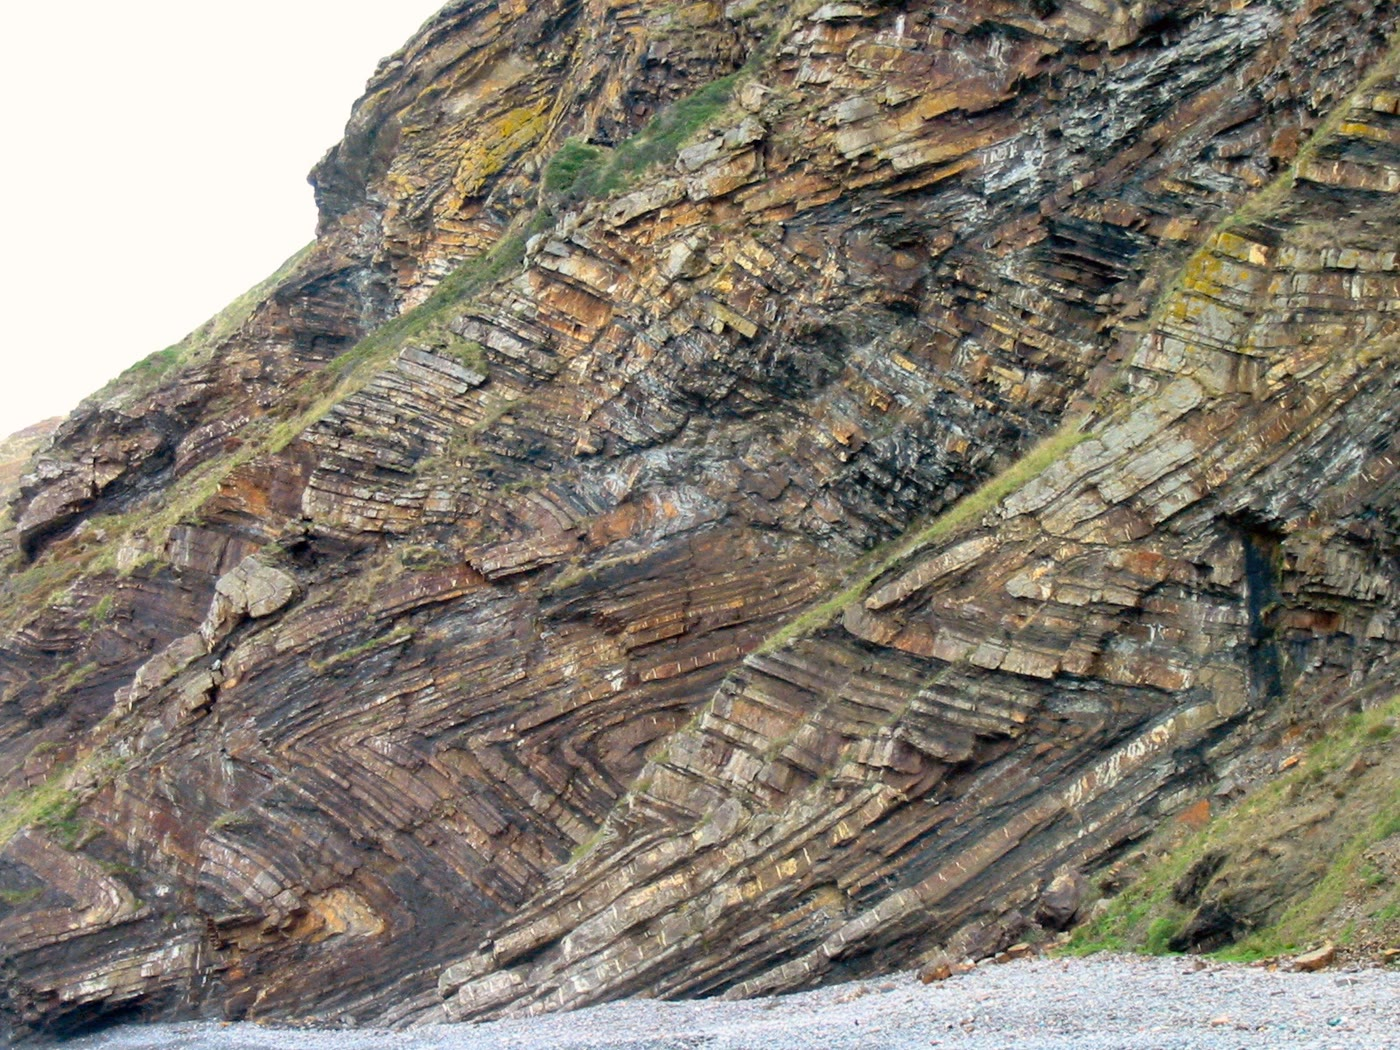
\includegraphics[width=0.78\linewidth]{images/book3/b1-chevron-folds-millook.jpg}
\par\smallskip{\small Geplooide lagen van zandsteen en schalie in de kliffen bij Millook, Noord-Cornwall: chevronplooien met bijna rechte \omterm{def:b1:faults-folds-fabrics:fold-elements}{flanken} en scherpe \omterm{def:b1:faults-folds-fabrics:fold-elements}{scharnieren}, hun axiale vlakken bijna verticaal. Foto: Smalljim, CC~BY~3.0
(Wikimedia Commons).}
\label{fig:b1:faults-folds-fabrics:chevrons}
\end{omfigure}
% ledger: commons:millook

\section{Structuren}\label{sec:b1:faults-folds-fabrics:fabrics}

Een vervormd gesteente is vaak door en door vervormd, niet alleen op enkele oppervlakken: zijn korrels zijn platgedrukt, gedraaid of hergroeid in een gemeenschappelijke oriëntatie, wat het een structuur geeft. Een vlakke structuur laat de rots splijten, een lineaire laat haar in staafjes breken.

\begin{definition}[Foliatie, schistositeit, leiklievage, axiaalvlakklievage]\label{def:b1:faults-folds-fabrics:foliation}
Een \emph{foliatie}\index{foliatie} is een vlakke structuur die een gesteente doordringt: een reeks dicht opeen liggende evenwijdige vlakken, gemaakt door uitgelijnde platte of afgeplatte korrels of door dunne lagen, waarlangs het gesteente het makkelijkst splijt.
\emph{Schistositeit}\index{schistositeit} is de foliatie van een schist, gemaakt door uitgelijnde korrels die grover zijn dan ongeveer \qty{1}{mm}. Een \emph{klievage}\index{klievage (van een gesteente)} is een foliatie van een fijnkorrelig gesteente die door zijn vervorming is ontstaan; \emph{leiklievage}\index{leiklievage} is de klievage van een leisteen, gemaakt door schilfermineralen die te klein zijn om met het blote oog te zien, en zo dicht opeen gezet dat het gesteente bijna overal in dunne platen kan worden gespleten. Een \emph{axiaalvlakklievage}\index{axiaalvlakklievage} is een klievage die evenwijdig is, of bijna evenwijdig, aan de axiale vlakken van de \omterm{def:b1:geological-maps:fold}{plooien} in dezelfde gesteenten.
\end{definition}
% ledger: ws:fabrics

Een \omterm{def:b1:faults-folds-fabrics:foliation}{foliatie} ontstaat ongeveer loodrecht op de richting van de grootste verkorting, door het draaien van schilferige korrels, de groei van nieuwe \omterm{def:b1:rock-forming-minerals:groups}{micas} en het oplossen van korrels op de vlakken die het sterkst worden samengedrukt. De \omterm{def:b1:faults-folds-fabrics:foliation}{klievage} van een leisteen heeft dus niets te maken met de gelaagdheid van de modder: zij legt de samenpersing vast. Wanneer \omterm{def:b1:geological-maps:fold}{plooien} en \omterm{def:b1:faults-folds-fabrics:foliation}{klievage} in dezelfde verkorting groeien, ligt de \omterm{def:b1:faults-folds-fabrics:foliation}{klievage} dicht bij de axiale vlakken van de \omterm{def:b1:geological-maps:fold}{plooien}, en waaiert zij er licht overheen uit, convergerend of divergerend naargelang de sterkte van elke laag, zoals de foto hieronder laat zien.
% ledger: ws:fabrics

\begin{omfigure}
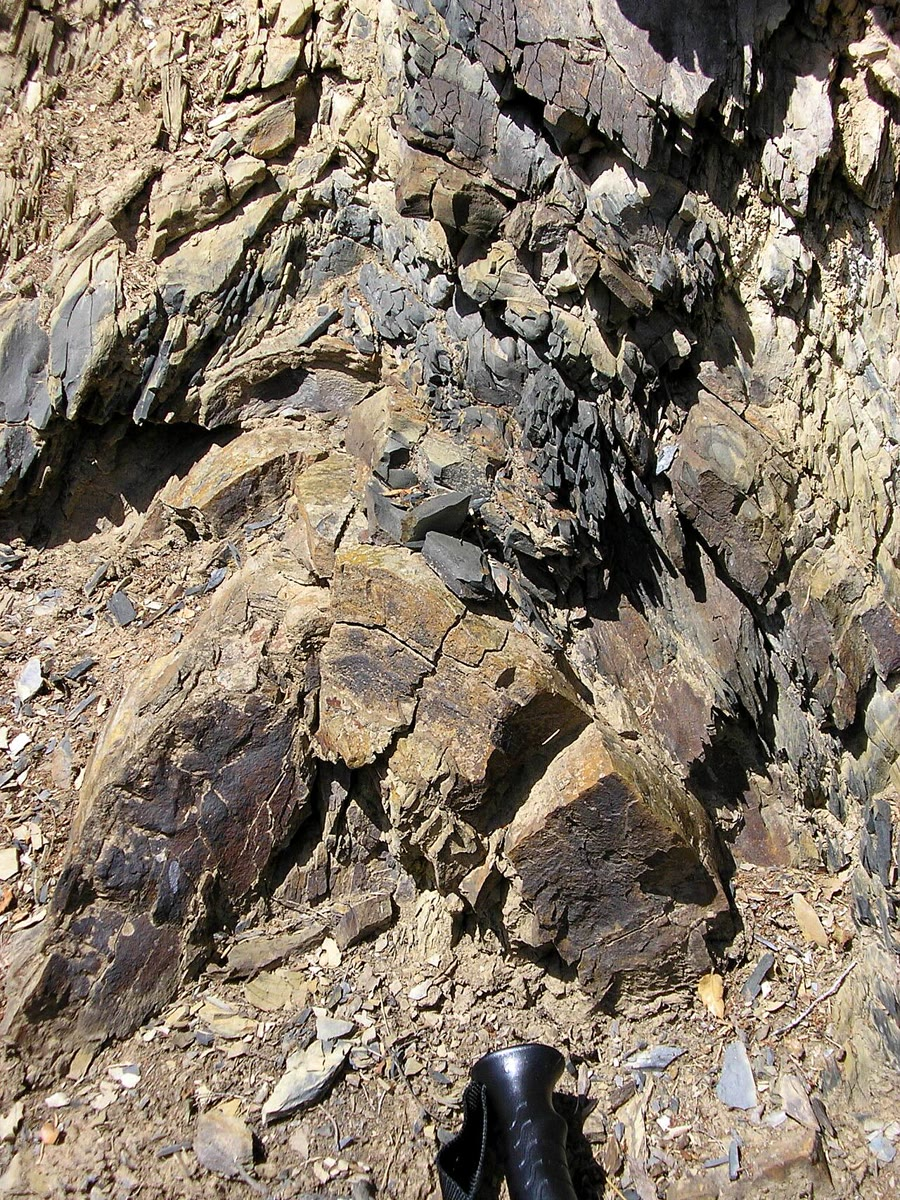
\includegraphics[height=8.2cm]{images/book3/b1-axial-planar-cleavage.jpg}
\par\smallskip{\small Een kleine \omterm{def:b1:geological-maps:fold}{antiklinaal} in afwisselend zandsteen en schalie van Carboon-ouderdom, bij Potes, Cantabrië. De bruine zandsteenlagen welven over het \omterm{def:b1:faults-folds-fabrics:fold-elements}{scharnier} onderin het midden van de foto; in de donkere schalie erboven is de \omterm{def:b1:faults-folds-fabrics:foliation}{klievage}, een reeks steile, dicht opeen liggende breuken die de lagen kruisen, axiaalvlakkig: bijna evenwijdig aan het axiale vlak van de \omterm{def:b1:geological-maps:fold}{plooi}, waaiert zij er overheen uit, en wisselt de waaier van laag tot laag. De handgreep van de wandelstok is ongeveer \qty{4}{cm} breed. Foto: Mikenorton, CC~BY-SA~3.0 (Wikimedia Commons).}
\label{fig:b1:faults-folds-fabrics:cleavage}
\end{omfigure}
% ledger: commons:axial-cleavage

\begin{definition}[Lineatie, snijlineatie, rekkingslineatie]\label{def:b1:faults-folds-fabrics:lineation}
Een \emph{lineatie}\index{lineatie} is een lineaire structuur die een gesteente doordringt, gemeten door haar richting en \omterm{def:b1:field-lab-methods-1:trend-plunge}{duik}. Een \emph{snijlineatie}\index{snijlineatie} is de verzameling lijnen waarin twee vlakke structuren elkaar snijden, zoals de gelaagdheid en een \omterm{def:b1:faults-folds-fabrics:foliation}{klievage}; een \emph{rekkingslineatie}\index{rekkingslineatie} bestaat uit korrels of stenen die langs de richting van de grootste rek zijn uitgetrokken.
\end{definition}
% ledger: ws:fabrics

\begin{proposition}[De snijlineatie van een plooi]\label{prop:b1:faults-folds-fabrics:intersection}
In een \omterm{def:b1:faults-folds-fabrics:fold-elements}{cilindrische plooi} met een \omterm{def:b1:faults-folds-fabrics:foliation}{axiaalvlakklievage} is de \omterm{def:b1:faults-folds-fabrics:lineation}{snijlineatie} van de gelaagdheid en de \omterm{def:b1:faults-folds-fabrics:foliation}{klievage} evenwijdig aan de \omterm{def:b1:faults-folds-fabrics:fold-elements}{scharnierlijn}, overal op de \omterm{def:b1:geological-maps:fold}{plooi}.
\end{proposition}

\begin{proof}
Elk gelaagdheidsvlak van een \omterm{def:b1:faults-folds-fabrics:fold-elements}{cilindrische plooi} bevat de richting van haar as. Het axiale vlak bevat de \omterm{def:b1:faults-folds-fabrics:fold-elements}{scharnierlijnen}, die evenwijdig zijn aan de as, dus bevat het die richting ook, en dat doet elk klievagevlak evenwijdig eraan. Twee vlakken die niet evenwijdig zijn en beide dezelfde richting bevatten, snijden elkaar langs een lijn van die richting.
\end{proof}

De stelling is de manier van de veldgeoloog om de \omterm{def:b1:field-lab-methods-1:trend-plunge}{duik} van een \omterm{def:b1:geological-maps:fold}{plooi} te vinden die te groot is om in één keer te zien: op elke \omterm{def:b1:geological-maps:geological-map}{ontsluiting} van een van beide \omterm{def:b1:faults-folds-fabrics:fold-elements}{flanken} geven de lijnen waarin de \omterm{def:b1:faults-folds-fabrics:foliation}{klievage} de gelaagdheid snijdt, de \omterm{def:b1:faults-folds-fabrics:fold-elements}{scharnierlijn}. De gelaagdheid en de \omterm{def:b1:faults-folds-fabrics:foliation}{klievage} samen zeggen meer: waar de \omterm{def:b1:geological-maps:fold}{plooi} is, en welke kant de lagen op staan.

\begin{definition}[Vergentie]\label{def:b1:faults-folds-fabrics:vergence}
De \emph{vergentie}\index{vergentie} van een asymmetrische \omterm{def:b1:geological-maps:fold}{plooi} is de horizontale richting waarnaar haar bovenste deel ten opzichte van haar onderste deel is verschoven: de richting waarin zij is overgekanteld of, voor een \omterm{def:b1:faults-folds-fabrics:fold-classes}{schuine plooi}, waarnaar zij hangt.
\end{definition}
% ledger: ws:vergence

\begin{proposition}[Gelaagdheid en klievage op de flanken van een plooi]\label{prop:b1:faults-folds-fabrics:cleavage-bedding}
Beschouw een \omterm{def:b1:geological-maps:fold}{plooi} met rechte \omterm{def:b1:faults-folds-fabrics:fold-elements}{flanken} en een \omterm{def:b1:faults-folds-fabrics:foliation}{axiaalvlakklievage}, in gesteenten die vóór de plooiing rechtop stonden, en waarin beide \omterm{def:b1:faults-folds-fabrics:fold-elements}{flanken} afdalen vanaf elk antiklinaalscharnier. In het profiel gezien:
\begin{enumerate}[label=(\alph*)]
  \item op een flank waar de gelaagdheid en de \omterm{def:b1:faults-folds-fabrics:foliation}{klievage} in dezelfde richting helen, is de gelaagdheid de steilste van de twee precies wanneer de flank is overgekanteld;
  \item de scherpe rotatie die de \omterm{def:b1:faults-folds-fabrics:foliation}{klievage} op de gelaagdheid draait, heeft op de twee \omterm{def:b1:faults-folds-fabrics:fold-elements}{flanken} van een \omterm{def:b1:geological-maps:fold}{plooi} tegengestelde zin; op een flank die niet is overgekanteld, verplaatst zij de top van de \omterm{def:b1:faults-folds-fabrics:foliation}{klievage} horizontaal naar het antiklinaalscharnier aan de top van die flank.
\end{enumerate}
\end{proposition}

\begin{proof}
Kijk langs het \omterm{def:b1:faults-folds-fabrics:fold-elements}{scharnier} met het axiale vlak dat naar links helt onder de hoek $\gamma$, $0 < \gamma \le \ang{90}$, en tel hoeken tegen de klok in vanaf de horizontale naar rechts. De \omterm{def:b1:faults-folds-fabrics:foliation}{klievage}, evenwijdig aan het axiale vlak, loopt omhoog onder de hoek $\gamma$. Bij een antiklinaalscharnier verlaten de twee \omterm{def:b1:faults-folds-fabrics:fold-elements}{flanken} naar beneden de hoeken $\ang{180} + \gamma - \iota/2$ (flank~1) en $\ang{180} + \gamma + \iota/2$ (flank~2), aan weerszijden van het axiale vlak, met $\iota/2 \le \gamma$ omdat beide dalen; elke flank van een reeks \omterm{def:b1:geological-maps:fold}{plooien} is een van deze twee voor de \omterm{def:b1:geological-maps:fold}{antiklinaal} aan haar top. De gesteenten worden jonger naar buiten, weg van de kern van de \omterm{def:b1:geological-maps:fold}{antiklinaal}, langs de normaal op de flank die van het axiale vlak af wijst.

Flank~1 gaat naar beneden naar links: zij helt naar links onder $\gamma - \iota/2$, minder steil dan de \omterm{def:b1:faults-folds-fabrics:foliation}{klievage}. Haar naar buiten gerichte normaal, onder $\ang{90} + \gamma -
\iota/2$, wijst omhoog: zij staat rechtop. Omhoog lopend maakt zij de hoek $\gamma - \iota/2$, dus de scherpe rotatie van de \omterm{def:b1:faults-folds-fabrics:foliation}{klievage} naar de gelaagdheid is met de klok mee, over $\iota/2$: de top van de \omterm{def:b1:faults-folds-fabrics:foliation}{klievage} verschuift naar rechts, waar het \omterm{def:b1:faults-folds-fabrics:fold-elements}{scharnier} is, omdat de flank het \omterm{def:b1:faults-folds-fabrics:fold-elements}{scharnier} naar links verlaat.

Flank~2 maakt met de horizontale, omhoog, de hoek $\gamma + \iota/2$. Als $\gamma + \iota/2 > \ang{90}$, gaat zij naar beneden naar rechts en helt zij naar rechts, tegengesteld aan de \omterm{def:b1:faults-folds-fabrics:foliation}{klievage}; haar naar buiten gerichte normaal, onder $\ang{270} + \gamma +
\iota/2$, heeft de opwaartse component $-\cos(\gamma + \iota/2) > 0$: zij staat rechtop. Als $\gamma + \iota/2 < \ang{90}$, gaat zij naar beneden naar links en helt zij naar links onder $\gamma + \iota/2$, steiler dan de \omterm{def:b1:faults-folds-fabrics:foliation}{klievage}, en is dezelfde component negatief: de flank is overgekanteld. In beide gevallen is de scherpe rotatie van de \omterm{def:b1:faults-folds-fabrics:foliation}{klievage} naar de gelaagdheid tegen de klok in, over $\iota/2$, en verplaatst zij de top van de \omterm{def:b1:faults-folds-fabrics:foliation}{klievage} naar links; wanneer de flank rechtop staat, verlaat zij het \omterm{def:b1:faults-folds-fabrics:fold-elements}{scharnier} naar rechts, dus ligt het \omterm{def:b1:faults-folds-fabrics:fold-elements}{scharnier} naar links. \omterm{def:b1:faults-folds-fabrics:fold-elements}{Flanken} die naar dezelfde kant helen als de \omterm{def:b1:faults-folds-fabrics:foliation}{klievage} zijn dus flank~1, minder steil, en een overgekantelde flank~2, steiler, en dat is (a); de zinnen zijn met de klok mee op flank~1 en tegen de klok in op flank~2, en dat is (b).
\end{proof}

De zin van de rotatie verandert dus bij elk \omterm{def:b1:faults-folds-fabrics:fold-elements}{scharnier}, \omterm{def:b1:geological-maps:fold}{antiklinaal} of \omterm{def:b1:geological-maps:fold}{synklinaal}.
Een geoloog die de zin langs een traject noteert, vindt de \omterm{def:b1:faults-folds-fabrics:fold-elements}{scharnieren} van \omterm{def:b1:geological-maps:fold}{plooien} die te groot zijn om in één \omterm{def:b1:geological-maps:geological-map}{ontsluiting} te zien waar de zin verandert, en de overgekantelde \omterm{def:b1:faults-folds-fabrics:fold-elements}{flanken} waar de gelaagdheid steiler is dan de \omterm{def:b1:faults-folds-fabrics:foliation}{klievage}; het woord \omterm{def:b1:faults-folds-fabrics:vergence}{vergentie} wordt ook voor deze zin van rotatie gebruikt, en de omkeringen van de \omterm{def:b1:faults-folds-fabrics:vergence}{vergentie} van kleine \omterm{def:b1:geological-maps:fold}{plooien} worden op dezelfde manier in kaart gebracht om de \omterm{def:b1:faults-folds-fabrics:fold-elements}{scharnieren} van grote \omterm{def:b1:geological-maps:fold}{plooien} te vinden: de kleine \omterm{def:b1:geological-maps:fold}{plooien} op de twee \omterm{def:b1:faults-folds-fabrics:fold-elements}{flanken} van een grote hebben tegengestelde asymmetrieën, en haar axiale spoor loopt tussen hen in.
% ledger: ws:vergence, ws:fold-elements

\begin{omfigure}
\begin{tikzpicture}[>={Stealth[length=5pt]}, font=\small]
% a train of chevron folds seen along the hinge (north into the page, east to the right):
% axial planes dipping 60 deg to the west, interlimb angle 40 deg; long limbs dip 40 deg W
% (the right way up), short limbs 80 deg W (overturned). Short limb: from an anticline hinge H_k,
% length s along 260 deg to the syncline hinge S_k; long limb back up along 40 deg to H_{k+1},
% so that all anticline hinges are level, a wavelength w apart.
% Five bedding surfaces, repeated along the axial direction (similar folds); cleavage parallel to it.
\def\s{2.6}
\pgfmathsetmacro{\sx}{\s*cos(260)}\pgfmathsetmacro{\sy}{\s*sin(260)}
\pgfmathsetmacro{\w}{\sx - \sy/tan(40)}
\pgfmathsetmacro{\hx}{0.62*cos(60)}\pgfmathsetmacro{\hy}{0.62*sin(60)}
\newcommand{\surface}[1]{%
  (-\w+#1*\hx, #1*\hy) \foreach \k in {-1,0,1,2,3} { -- ({\k*\w+\sx+#1*\hx}, {\sy+#1*\hy}) -- ({(\k+1)*\w+#1*\hx}, {#1*\hy}) }}
\begin{scope}
  \clip (0.35,-3.3) rectangle (10.0,2.95);
  \begin{scope}
    \clip \surface{0} -- (12,6) -- (-4,6) -- cycle;
    \clip \surface{4} -- (12,-6) -- (-4,-6) -- cycle;
    \fill[omLithSand!45] (-4,-6) rectangle (12,6);
    \fill[omLithShale!40] \surface{2} -- (12,6) -- (-4,6) -- cycle;
    \fill[omLithSand!45] \surface{3} -- (12,6) -- (-4,6) -- cycle;
    \foreach \c in {-8.0,-7.78,...,13.0} {
      \draw[omDef!85, line width=0.35pt] ({\c-6*cot(60)},-6) -- ({\c+6*cot(60)},6);
    }
  \end{scope}
  \foreach \j in {0,1,2,3,4} { \draw[line width=0.75pt, line join=round] \surface{\j}; }
\end{scope}
% axial traces through the anticline hinges, and labels
\foreach \k in {1,2,3} {
  \draw[omThm, dashed, line width=0.6pt] ({\k*\w-0.5*cos(60)},{-0.5*sin(60)}) -- ({\k*\w+3.6*cos(60)},{3.6*sin(60)});
  \node[omThm, font=\scriptsize, anchor=south] at ({\k*\w+3.6*cos(60)},{3.6*sin(60)}) {antiklinaal};
}
\foreach \k in {1,2,3} { \node[omThm, font=\scriptsize, anchor=north] at ({\k*\w+\sx},{\sy-0.15}) {synklinaal}; }
\end{tikzpicture}
\par\smallskip{\small Een reeks chevronplooien, in profiel overgekanteld naar rechts, met een \omterm{def:b1:faults-folds-fabrics:foliation}{axiaalvlakklievage} (dunne blauwe lijnen), op schaal getekend: axiale vlakken die \ang{60} naar links hellen, \omterm{def:b1:faults-folds-fabrics:fold-elements}{interflankhoek} \ang{40}. De lange \omterm{def:b1:faults-folds-fabrics:fold-elements}{flanken} helen \ang{40} naar links, minder steil dan de \omterm{def:b1:faults-folds-fabrics:foliation}{klievage}, en staan rechtop; de korte \omterm{def:b1:faults-folds-fabrics:fold-elements}{flanken} helen \ang{80} naar links, steiler dan de \omterm{def:b1:faults-folds-fabrics:foliation}{klievage}, en zijn overgekanteld. De scherpe hoek waarmee de \omterm{def:b1:faults-folds-fabrics:foliation}{klievage} op de gelaagdheid wordt gedraaid, is op elke lange flank met de klok mee en op elke korte flank tegen de klok in. De \omterm{def:b1:geological-maps:fold}{plooien} zijn naar rechts vergent.}
\label{fig:b1:faults-folds-fabrics:vergence}
\end{omfigure}

\section{Microstructuren}\label{sec:b1:faults-folds-fabrics:micro}

Onder de microscoop toont de vervorming van een gesteente zich in zijn korrels. Een kwartskorrel die door het langzame glijden van zijn kristalrooster is gebogen, gaat niet meer in één keer uit in \omterm{def:b1:field-lab-methods-1:microscope}{gekruiste polarisatoren}: wanneer het stadium draait, schuift een donkere band erover, omdat haar delen in iets andere richtingen wijzen. Deze golvende uitdoving (\cref{ch:b1:optical-mineralogy}) wordt sterker naarmate men een schuifzone nadert, omdat defecten zich in het kristalrooster opstapelen. Waar water aanwezig is, lossen korrels op op de vlakken waar zij het sterkst worden samengedrukt, en wordt de opgeloste stof afgezet waar de spanning lager is, of weggevoerd: deze drukoplossing verkort gesteenten bij lage temperatuur en vormt veel \omterm{def:b1:faults-folds-fabrics:foliation}{klievages}. Bij hogere temperatuur worden de vervormde korrels vervangen, terwijl de vervorming doorgaat, door nieuwe, kleinere en onvervormde korrels, eerst langs de oude korrelgrenzen: dynamische herkristallisatie, die de korrelgrootte verkleint en mylonieten maakt. De vormen van vervormde korrels en van de mineralen die in hun drukschaduw groeien, tonen ook welke kant een schuifzone op is gegaan; deze indicatoren van de schuifzin en de mechanismen zelf horen thuis in Boek~5.
% ledger: ws:microstructures, ws:fabrics

\section{Oefeningen}

\begin{exercise}[$\star$]\label{exo:b1:faults-folds-fabrics:1}
Benoem elke breuk aan de hand van de \omterm{def:b1:faults-folds-fabrics:fault-elements}{rake} van haar \omterm{def:b1:faults-folds-fabrics:fault-elements}{verschuivingsvector}, van het vlak dat \ang{60} helt:
(a) $r = \ang{-90}$; (b) $r = \ang{85}$; (c) $r = 0$; (d) $r = \ang{180}$;
(e) $r = \ang{-40}$. (f) Geef de naam van (b) als de helling \ang{25} was.
% ledger: ar:rake, usgs:fault-types
\end{exercise}

\begin{exercise}[$\star$]\label{exo:b1:faults-folds-fabrics:2}
Een \omterm{def:b1:faults-folds-fabrics:fault-types}{normaalbreuk} helt \ang{55}; haar verschuiving is zuiver dip-slip, met een \omterm{def:b1:faults-folds-fabrics:fault-elements}{netto verschuiving} van \qty{300}{m}. Bereken haar \omterm{def:b1:cross-sections:throw}{worp} en haar \omterm{def:b1:cross-sections:throw}{horizontale verplaatsing}.
\end{exercise}

\begin{exercise}[$\star$]\label{exo:b1:faults-folds-fabrics:3}
Geef de \omterm{def:b1:faults-folds-fabrics:fold-elements}{interflankhoek} en de klasse van elke \omterm{def:b1:faults-folds-fabrics:fold-classes}{rechtopstaande plooi}, waarvan de \omterm{def:b1:faults-folds-fabrics:fold-elements}{flanken} in tegengestelde richtingen helen: (a) \omterm{def:b1:faults-folds-fabrics:fold-elements}{flanken} die \ang{35} en \ang{35} helen; (b) \ang{70} en \ang{75}; (c) \ang{85} en \ang{88}.
% ledger: ws:fold-classes
\end{exercise}

\begin{exercise}[$\star$]\label{exo:b1:faults-folds-fabrics:4}
Een zandsteen heeft de \omterm{def:b1:stress-strain-rheology:coulomb}{inwendige wrijvingshoek} \ang{35}. Bepaal volgens de theorie van Anderson onder welke hoeken haar \omterm{def:b1:faults-folds-fabrics:fault-types}{normaalbreuken} en haar \omterm{def:b1:faults-folds-fabrics:fault-types}{overschuivingen} helen. Bereken de hoek die twee geconjugeerde \omterm{def:b1:faults-folds-fabrics:fault-types}{strike-slip-breuken} met elkaar maken.
\end{exercise}

\begin{exercise}[$\star\star$]\label{exo:b1:faults-folds-fabrics:5}
Een breuk heeft de ligging $090/50$, en op haar liggen \omterm{def:b1:faults-folds-fabrics:fault-rocks}{slickenlines} van \omterm{def:b1:faults-folds-fabrics:fault-elements}{rake} \ang{-30}; de \omterm{def:b1:faults-folds-fabrics:fault-elements}{netto verschuiving} is \qty{400}{m}. (a) Bereken de strike-slip- en dip-slip-componenten, de \omterm{def:b1:cross-sections:throw}{worp} en de \omterm{def:b1:cross-sections:throw}{horizontale verplaatsing}. (b) Schrijf de \omterm{def:b1:faults-folds-fabrics:fault-elements}{verschuivingsvector} in oost-, noord- en opwaartse componenten, en geef haar richting en \omterm{def:b1:field-lab-methods-1:trend-plunge}{duik}. (c) Benoem de breuk.
\end{exercise}

\begin{exercise}[$\star\star$]\label{exo:b1:faults-folds-fabrics:6}
Twee verticale \omterm{def:b1:faults-folds-fabrics:fault-types}{strike-slip-breuken} van dezelfde ouderdom lopen $020$ en $080$. (a) Geef volgens Anderson de richtingen van $\sigma_1$, $\sigma_2$ en $\sigma_3$, en de \omterm{def:b1:stress-strain-rheology:coulomb}{inwendige wrijvingshoek} van het gesteente. (b) Geef aan welke breuk \omterm{def:b1:faults-folds-fabrics:fault-types}{dextraal} en welke \omterm{def:b1:faults-folds-fabrics:fault-types}{sinistraal} is. Argumenteer uit de verkorting langs $\sigma_1$.
\end{exercise}

\begin{exercise}[$\star\star$]\label{exo:b1:faults-folds-fabrics:7}
De twee \omterm{def:b1:faults-folds-fabrics:fold-elements}{flanken} van een \omterm{def:b1:faults-folds-fabrics:fold-elements}{cilindrische plooi} hebben de ligging $120/40$ en $260/30$. Bepaal met \cref{prop:b1:faults-folds-fabrics:hinge} de richting en \omterm{def:b1:field-lab-methods-1:trend-plunge}{duik} van haar \omterm{def:b1:faults-folds-fabrics:fold-elements}{scharnierlijn}, haar \omterm{def:b1:faults-folds-fabrics:fold-elements}{interflankhoek} en haar klasse.
\end{exercise}

\begin{exercise}[$\star\star$]\label{exo:b1:faults-folds-fabrics:8}
Op een \omterm{def:b1:geological-maps:geological-map}{ontsluiting} heeft de gelaagdheid de ligging $040/30$ en de \omterm{def:b1:faults-folds-fabrics:foliation}{axiaalvlakklievage} de ligging $160/80$. Bepaal de richting en \omterm{def:b1:field-lab-methods-1:trend-plunge}{duik} van de \omterm{def:b1:faults-folds-fabrics:lineation}{snijlineatie}. Geef aan wat zij over de \omterm{def:b1:geological-maps:fold}{plooi} zegt.
\end{exercise}

\begin{exercise}[$\star\star$]\label{exo:b1:faults-folds-fabrics:9}
Een verticale breuk loopt oost--west. Een verticale gang die noord--zuid loopt, snijdt haar; ten noorden van de breuk wordt de gang \qty{350}{m} oostwaarts gevonden van waar zij ten zuiden van de breuk is. (a) Is de breuk \omterm{def:b1:faults-folds-fabrics:fault-types}{dextraal} of \omterm{def:b1:faults-folds-fabrics:fault-types}{sinistraal}? (b) Als de \omterm{def:b1:faults-folds-fabrics:fault-rocks}{slickenlines} horizontaal zijn, bepaal de \omterm{def:b1:faults-folds-fabrics:fault-elements}{netto verschuiving}. (c) Als zij in plaats daarvan een \omterm{def:b1:field-lab-methods-1:trend-plunge}{duik} van \ang{20} naar het oosten hebben, bepaal de \omterm{def:b1:faults-folds-fabrics:fault-elements}{netto verschuiving} en de verticale component van de verschuiving, en geef aan welk blok omlaag is gegaan.
\end{exercise}

\begin{exercise}[$\star\star\star$]\label{exo:b1:faults-folds-fabrics:10}
Een breuk zonder \omterm{def:b1:stress-strain-rheology:coulomb}{cohesie} met wrijvingscoëfficiënt $\mu$ maakt de hoek $\theta$ met $\sigma_1$. (a) Toon aan dat zij glijdt wanneer de effectieve \omterm{def:b1:stress-strain-rheology:principal}{hoofdspanningen} de verhouding bereiken
\[
  \frac{\sigma_1'}{\sigma_3'} = \frac{1 + \mu\cot\theta}{1 - \mu\tan\theta} .
\]
(b) Met $\mu = 0.6$ en $\sigma_1$ verticaal, bereken de verhouding voor \omterm{def:b1:faults-folds-fabrics:fault-types}{normaalbreuken} die \ang{60}, \ang{45} en \ang{35} helen. (c) Toon aan dat een \omterm{def:b1:faults-folds-fabrics:fault-types}{normaalbreuk} die minder dan een bepaalde hoek helt, nooit kan glijden, en bereken die hoek. (d) Geef voor $\mu = 0.6$ en $\mu = 0.85$ de hellingen van de best georiënteerde \omterm{def:b1:faults-folds-fabrics:fault-types}{normaalbreuken} en \omterm{def:b1:faults-folds-fabrics:fault-types}{overschuivingen}.
\end{exercise}

\begin{exercise}[$\star\star\star$]\label{exo:b1:faults-folds-fabrics:11}
Langs een oost--west-traject over chevronplooien waarvan de \omterm{def:b1:faults-folds-fabrics:fold-elements}{scharnieren} noord lopen, helt een \omterm{def:b1:faults-folds-fabrics:foliation}{axiaalvlakklievage} overal \ang{60} naar het westen. De gelaagdheid helt \ang{40} W op station A, \ang{80} W op station B en \ang{40} W op station C, van west naar oost, in gesteenten die vóór de plooiing rechtop stonden. (a) Welk station ligt op een overgekantelde flank? (b) Bepaal in welke zin de \omterm{def:b1:faults-folds-fabrics:foliation}{klievage} op de gelaagdheid draait op elk station, gezien naar het noorden. (c) Bepaal waar de \omterm{def:b1:faults-folds-fabrics:fold-elements}{scharnieren} liggen, en welke antiklinalen zijn. (d) Bepaal de \omterm{def:b1:faults-folds-fabrics:fold-elements}{interflankhoek} en de ligging van de axiale vlakken, en geef aan naar welke kant de \omterm{def:b1:geological-maps:fold}{plooien} vergent zijn.
\end{exercise}

\begin{exercise}[$\star\star\star$]\label{exo:b1:faults-folds-fabrics:12}
Een laag van lengte $L_0$ wordt geplooid tot een reeks symmetrische chevronplooien met \omterm{def:b1:faults-folds-fabrics:fold-elements}{interflankhoek} $\iota$, met ongewijzigde lengte. (a) Toon aan dat haar lengte, gemeten over de \omterm{def:b1:geological-maps:fold}{plooien}, $L_0\sin(\iota/2)$ wordt. (b) Bepaal de verkorting die chevronplooien met een \omterm{def:b1:faults-folds-fabrics:fold-elements}{interflankhoek} van \ang{60} vertegenwoordigen. (c) Bepaal de \omterm{def:b1:faults-folds-fabrics:fold-elements}{interflankhoek} die hoort bij een verkorting van \qty{30}{\percent}. (d) Bepaal de verkorting van een reeks \omterm{def:b1:faults-folds-fabrics:fold-classes}{rechtopstaande plooien} met \omterm{def:b1:faults-folds-fabrics:fold-elements}{flanken} die \ang{12} helen.
\end{exercise}

\section{Probleem: de structuren van de Varden Hills, gemeten}

\begin{problem}[{Weekendprobleem --- de antiklinaal en de normaalbreuk van de Varden Hills, uit de liggingen van hun vlakken tot de verschuiving op de breuk}]
\label{pb:b1:faults-folds-fabrics:1}
% values: calc/ch17.py; region: figdata/shared/region.py (limbs, plunge, fault)
De Varden Hills zijn geplooid tot een \omterm{def:b1:geological-maps:fold}{antiklinaal}, waarvan de as noord--zuid loopt op $x = \qty{3.5}{km}$, en een \omterm{def:b1:geological-maps:fold}{synklinaal} \qty{4}{km} ten oosten ervan; beide hebben vlakke \omterm{def:b1:faults-folds-fabrics:fold-elements}{flanken}. Een veldmeting mat de gelaagdheid op de oostflank van de \omterm{def:b1:geological-maps:fold}{antiklinaal} als $080.7/12.2$ en op haar westflank als $279.3/12.2$. Het dek wordt doorsneden door een \omterm{def:b1:faults-folds-fabrics:fault-types}{normaalbreuk} met ligging $120/60$, waarvan de \omterm{def:b1:faults-folds-fabrics:fault-elements}{hangende wand} langs de helling omlaag is bewogen, met een \omterm{def:b1:cross-sections:throw}{worp} van \qty{200}{m}. Geef hoeken tot op \ang{0.1} en lengten tot op \qty{0.1}{m} nauwkeurig.

\medskip
\noindent\textbf{Deel I --- De flanken.}
\begin{enumerate}
  \item Schrijf de opwaartse eenheidsnormalen $\mathbf n_1$ (oostflank) en
        $\mathbf n_2$ (westflank) op, in oost-, noord- en opwaartse componenten.
  \item Bereken $\mathbf n_1\cdot\mathbf n_2$ en de hoek tussen de normalen.
  \item Leid de \omterm{def:b1:faults-folds-fabrics:fold-elements}{interflankhoek} van de \omterm{def:b1:geological-maps:fold}{antiklinaal} af.
  \item Classificeer de \omterm{def:b1:geological-maps:fold}{antiklinaal} naar haar \omterm{def:b1:faults-folds-fabrics:fold-elements}{interflankhoek}.
  \item De twee \omterm{def:b1:faults-folds-fabrics:fold-elements}{flanken} helen \ang{12.2}. Leg uit waarom de \omterm{def:b1:faults-folds-fabrics:fold-elements}{interflankhoek} niet precies $\ang{180} - 2\times\ang{12.2}$ is. Bereken de \omterm{def:b1:cross-sections:apparent-dip}{schijnbare helling} van beide \omterm{def:b1:faults-folds-fabrics:fold-elements}{flanken} in een oost--west-verticale doorsnede.
  \item De \omterm{def:b1:geological-maps:fold}{synklinaal} deelt de oostflank van de \omterm{def:b1:geological-maps:fold}{antiklinaal}, en haar eigen oostflank is evenwijdig aan de westflank van de \omterm{def:b1:geological-maps:fold}{antiklinaal}. Bepaal haar \omterm{def:b1:faults-folds-fabrics:fold-elements}{interflankhoek}.
\end{enumerate}

\medskip
\noindent\textbf{Deel II --- Het scharnier en het axiale vlak.}
\begin{enumerate}[resume]
  \item Bereken $\mathbf n_1\times\mathbf n_2$, en de richting en \omterm{def:b1:field-lab-methods-1:trend-plunge}{duik} van de \omterm{def:b1:faults-folds-fabrics:fold-elements}{scharnierlijn}.
  \item Geef de ligging van het axiale vlak en bepaal of de \omterm{def:b1:geological-maps:fold}{antiklinaal} rechtopstaand, schuin of liggend is.
  \item Geef de volledige beschrijving van de \omterm{def:b1:geological-maps:fold}{plooi}: strakheid, ligging van het axiale vlak, \omterm{def:b1:field-lab-methods-1:trend-plunge}{duik}.
  \item Geef op de \omterm{def:b1:geological-maps:geological-map}{geologische kaart} van \cref{ch:b1:geological-maps} aan in welke richting de \omterm{def:b1:geological-maps:geological-map}{ontsluitingen} van de \omterm{def:b1:geological-maps:fold}{antiklinaal} sluiten, en welk gesteente in haar kern ontsloten is.
  \item De schalie van het dek draagt een \omterm{def:b1:faults-folds-fabrics:foliation}{axiaalvlakklievage}. Geef haar ligging, en de richting en \omterm{def:b1:field-lab-methods-1:trend-plunge}{duik} van haar \omterm{def:b1:faults-folds-fabrics:lineation}{snijlineatie} op de oostflank.
  \item Geef op de oostflank de zin waarin de \omterm{def:b1:faults-folds-fabrics:foliation}{klievage} op de gelaagdheid draait, gezien naar het noorden, en aan welke kant het antiklinaalscharnier ligt.
\end{enumerate}

\medskip
\noindent\textbf{Deel III --- De breuk en de spanningen.}
\begin{enumerate}[resume]
  \item Geef de \omterm{def:b1:geological-maps:attitude}{strijk} van de breuk volgens de rechterhandregel, en zeg aan welke kant van haar spoor de \omterm{def:b1:faults-folds-fabrics:fault-elements}{hangende wand} ligt.
  \item Bepaal welke hoofdspanning verticaal was toen de breuk ontstond, volgens Anderson.
  \item Geef de richtingen van de twee horizontale \omterm{def:b1:stress-strain-rheology:principal}{hoofdspanningen}.
  \item Bepaal welke \omterm{def:b1:stress-strain-rheology:coulomb}{inwendige wrijvingshoek} de helling impliceert, en de bijbehorende wrijvingscoëfficiënt.
  \item Geef de ligging van de geconjugeerde set breuken die dezelfde spanningen zouden hebben kunnen maken, en de hoek tussen de twee sets.
  \item Bepaal of de breuk onder hetzelfde regime opnieuw het best georiënteerd is om te glijden, met de wrijving van Byerlee van 0.85.
\end{enumerate}

\medskip
\noindent\textbf{Deel IV --- De verschuiving.}
\begin{enumerate}[resume]
  \item Geef de \omterm{def:b1:faults-folds-fabrics:fault-elements}{rake} van de \omterm{def:b1:faults-folds-fabrics:fault-elements}{verschuivingsvector}, en haar richting en \omterm{def:b1:field-lab-methods-1:trend-plunge}{duik}.
  \item Schrijf de eenheidsvector van de verschuiving in oost-, noord- en opwaartse componenten.
  \item Bereken de \omterm{def:b1:cross-sections:throw}{horizontale verplaatsing} (\omterm{def:b1:cross-sections:throw}{heave}) van de breuk.
  \item Bereken de oost- en noordcomponenten van de \omterm{def:b1:cross-sections:throw}{horizontale verplaatsing} van de \omterm{def:b1:faults-folds-fabrics:fault-elements}{hangende wand}.
  \item Controleer dat de \omterm{def:b1:faults-folds-fabrics:fault-elements}{netto verschuiving} $L$, de \omterm{def:b1:cross-sections:throw}{worp} $h$ en de \omterm{def:b1:cross-sections:throw}{horizontale verplaatsing} $e$ voldoen aan $L^2 = h^2 + e^2$, en leg uit waarom.
  \item Bepaal, op de meter nauwkeurig, de \omterm{def:b1:faults-folds-fabrics:fault-elements}{netto verschuiving} van de breuk van de Varden Hills.
\end{enumerate}
\end{problem}
